\chapter{LEARNING FROM OFFLINE AND ONLINE DATA}
\label{ch:hybrid-rl}

\todoresolve{CHAPTER 2 COMBINES TWO HYBRID RL PAPERS (SECTIONS 2.1-2.3: TAN AND XU 2024; SECTIONS 2.4-2.10: TAN, FAN, AND WEI 2024). AI-WRITTEN CHAPTER OVERVIEW, BRIDGE PARAGRAPHS, AND ALGORITHM-NAME REPLACEMENTS ARE IN GREEN.}

\begin{aigenblock}

Reinforcement learning (RL) encompasses two main paradigms distinguished by how training data are acquired: online RL and offline RL. In online RL, an agent interacts with the environment in real time and executes a sequence of adaptively chosen policies to maximize cumulative reward \citep{sutton1998, azar2017minimax, jin2018q, zhang2023settling}. In offline RL, the agent has access only to a pre-collected dataset logged by a behavior policy and seeks a near-optimal policy without further environmental interaction \citep{lange2012batch, levine2020offline, jin2021pessimism, li2024settling}. Purely online methods often require an impractically large number of interactive trajectories, whereas purely offline methods impose stringent coverage assumptions on the pre-collected dataset, typically requiring single-policy concentrability with respect to an optimal policy \citep{rashidinejad2021bridging, zhan2022offline, xie2021bellman}.

Hybrid reinforcement learning combines offline datasets with online environmental interaction \citep{vecerik2017leveraging, nair2020awac, xie2022policy, song2023hybrid, nakamoto2023calql, wagenmaker2023leveraging, li2023reward, ball2023efficient, zhou2023offline, amortila2024harnessing}. A central theoretical question posed by \citet{xie2022policy} is whether hybrid RL can provably improve upon both purely offline and purely online learning when the offline dataset lacks single-policy concentrability. Indeed, \citet{xie2022policy} proved that if the behavior policy already satisfies single-policy concentrability and the learner can choose the ratio of offline to online trajectories, then either purely offline learning or purely online learning is minimax optimal, leaving no statistical advantage to combining both sources. Consequently, the regime in which hybrid RL offers genuine statistical gains is precisely when the offline dataset has only partial coverage of the state-action space, so that online interaction must fill in the regions left unexplored by the behavior policy.

This chapter develops the statistical theory and algorithmic design of hybrid RL without single-policy concentrability across two settings:
\begin{enumerate}
    \item \textbf{General function approximation via experience replay initialization (Sections~\ref{sec:ch02-gfa-setup}--\ref{sec:ch02-gfa-sims}):} Based on joint work with Ziping Xu \citep{tan2024natural}, we show that warm-starting an optimistic general function approximation algorithm by appending the entire offline dataset to its experience replay buffer (Algorithm~\ref{alg:ch02-alg1}) achieves regret guarantees that adapt automatically to the best partition of the state-action space into an offline-covered subset $\gX_{\off}$ and an online-explored subset $\gX_{\on}$, without the algorithm ever knowing or estimating the partition. We further establish a general conversion recipe (Proposition~\ref{prop:ch02-general_recipe}) and specialize the resulting guarantees to tabular, linear, and block Markov decision processes.
    \item \textbf{Breaking sample-size barriers in linear MDPs (Sections~\ref{sec:ch02-lin-intro}--\ref{sec:ch02-lin-discussion}):} While general function approximation yields broad adaptivity, its squared-Bellman-error confidence sets incur suboptimal $H^5$ horizon dependence when specialized to linear MDPs. Based on joint work with Wei Fan and Yuting Wei \citep{tan2024hybrid}, we develop two computationally efficient algorithms tailored to linear MDPs that sharpen both the dimension dependence and the horizon dependence to $H^3$. The first method, Algorithm~\ref{alg:ch02-alg2}, follows an online-to-offline design that uses reward-agnostic covariate collection \citep{wagenmaker2023instancedependent} followed by variance-weighted pessimistic value iteration \citep{xiong2023nearly} to output a fixed policy with near-optimal PAC suboptimality. The second method, Algorithm~\ref{alg:ch02-alg3}, follows an offline-to-online design that warm-starts variance-weighted optimistic value iteration \citep{he2023nearly} with offline parameter estimates to achieve sublinear online regret that improves upon the minimax lower bound for purely online linear MDPs whenever offline data cover a nontrivial subspace.
\end{enumerate}
All proofs and supplementary experimental figures for this chapter are presented in Appendix~\ref{app:ch02}.


\end{aigenblock}

% =========================================================================
% PART 1: GENERAL FUNCTION APPROXIMATION (Tan and Xu, 2024)
% =========================================================================

\section{Hybrid RL with General Function Approximation}
\label{sec:ch02-gfa-setup}

Many online RL algorithms explore by maintaining an experience replay buffer and minimizing empirical Bellman error over the collected transitions to update confidence sets or value estimates \citep{auer2008near, jin2021bellmaneluder, xie2022role}. A natural way to extend such an online algorithm to the hybrid setting is to include the offline dataset in the replay buffer from the start \citep{song2023hybrid, nakamoto2023calql, amortila2024harnessing}. Prior analyses of this replay-initialization strategy required single-policy concentrability over the entire state-action space and discarded offline trajectories whenever $N_{\off} > N_{\on}$. Meanwhile, the works that avoided single-policy concentrability \citep{li2023reward, wagenmaker2023leveraging} relied on multi-stage reward-free Frank--Wolfe exploration subroutines rather than direct online regret minimization.

We show that simply appending the entire offline dataset to the replay buffer of an optimistic squared-Bellman-error algorithm \citep{jin2021bellmaneluder, xie2022role} yields provable improvements over both pure online and pure offline learning even when the offline dataset has arbitrarily poor coverage. We establish this by considering arbitrary (not necessarily disjoint) partitions $\gX_{\off} \cup \gX_{\on} = \gX$ of the state-action-horizon space, bounding the regret on $\gX_{\off}$ via a partial offline concentrability coefficient and the regret on $\gX_{\on}$ via a restricted online sequential extrapolation coefficient, and taking the infimum over all partitions $\gX_{\off}, \gX_{\on}$.

\paragraph{Notation.}
Let $\gN_{\gF}(\rho)$ denote the $\rho$-covering number of a function class $\gF$ with respect to the supremum norm. Let $N_{\off}$ and $N_{\on}$ (with $N = N_{\off} + N_{\on}$) denote the number of episodes in the offline dataset and the number of online episodes, respectively. We use $T = N_{\on}$ interchangeably when referring to the online horizon. For any subset $\gX' \subset \gS \times \gA \times [H]$, let $\gX'_h = \{(s, a) \in \gS \times \gA: (s, a, h) \in \gX'\}$, and let $\Delta(\gY)$ denote the set of probability distributions over $\gY$.

\paragraph{Episodic MDPs.}
We consider episodic Markov decision processes denoted by $\gM = (\gS, \gA, H, P, R)$, where $\gS$ is the state space, $\gA$ is the action space, $H$ is the episode horizon, $P = \{P_h\}_{h \in [H]}$ is the collection of transition probability kernels with $P_h: \gS \times \gA \mapsto \Delta(\gS)$, and $R = \{R_h\}_{h \in [H]}$ is the collection of deterministic reward functions with $R_h: \gS \times \gA \mapsto [0, 1]$. Within each episode, at step $h \in [H]$, the agent observes state $s_h \in \gS$, selects action $a_h \in \gA$, receives reward $r_h = R_h(s_h, a_h)$, and transitions to $s_{h+1} \sim P_h(\cdot \mid s_h, a_h)$. A policy $\pi = \{\pi_h\}_{h \in [H]}$ maps states to distributions over actions. A value-function class $\gF = \{\gF_h\}_{h \in [H]}$ induces a greedy policy class $\Pi \coloneqq \{\pi^f : f\in \gF\}$, where $\pi^f_h(s) = \argmax_{a \in \gA} f_h(s, a)$. Throughout Sections~\ref{sec:ch02-gfa-setup}--\ref{sec:ch02-gfa-sims}, we write $\gX = \gS \times \gA \times [H]$.

\begin{defn}[Occupancy Measure]
\label{defn:ch02-occ}
The occupancy measure $d^{\pi} = \{d^{\pi}_h\}_{h = 1}^H$ is the collection of state-action distributions induced by executing policy $\pi$ in $\gM$, where $d^\pi_h(s,a) = \mathbb{P}(s_h = s, a_h = a \mid \pi)$. We write $\sD = \{d^\pi : \pi \in \Pi\}$ and $\sD_h = \{d^\pi_h : \pi \in \Pi\}$.
\end{defn}

\paragraph{Hybrid RL Interaction Protocol.}
In the offline-to-online fine-tuning protocol, the learner is given an offline dataset $\gD_{\off} = \{\gD_{\off, h}\}_{h=1}^H$ consisting of $N_{\off}$ episodes collected by a fixed behavior policy $\pi_{\off} = \{\pi_{\off, h}\}_{h \in [H]}$ with occupancy measure $\mu = \{\mu_h\}_{h=1}^H$, and subsequently interacts with the environment for $N_{\on}$ online episodes. Denote by $s_{h}^{(t)}$, $a_{h}^{(t)}$, and $r_{h}^{(t)}$ the state, action, and reward at step $h \in [H]$ of online episode $t \in [N_{\on}]$. For any policy $\pi$, its value function and action-value function at step $h$ are defined as
\begin{equation}
    V_{h}^{\pi}(s) = \E_{\pi}\!\left[\sum_{h' = h}^H r_{h'} \,\middle|\, s_{h} = s\right], \qquad
    Q^{\pi}_h(s, a) = \E_{\pi}\!\left[\sum_{h' = h}^H r_{h'} \,\middle|\, s_{h} = s, a_{h} = a\right],
\end{equation}
with $V_{H+1}^{\pi}(s) \equiv 0$. We write $V^{\star}$ and $Q^{\star}$ for the optimal value and action-value functions. The cumulative regret of an online learning algorithm $\gL$ over $N_{\on}$ episodes is
\begin{equation}
    \Reg(N_{\on}, \gL) = \E_{\gL}\!\left[\sum_{t = 1}^{N_{\on}}\left( V^\star_{1}(s_{1}^{(t)}) - \sum_{h = 1}^H r_{h}^{(t)} \right)\right].
\end{equation}

\paragraph{Function Approximation.}
We approximate $Q^\star$ using a function class $\gF = \{\gF_h\}_{h \in [H]}$ with $\gF_h \subseteq [0, H]^{\gS \times \gA}$ and $f_{H+1} \equiv 0$. For each $h \in [H]$, the Bellman optimality operator $\gT_h$ is defined by
\begin{equation}
    \gT_h f_{h+1}(s, a) \coloneqq R_h(s, a) + \E_{s' \sim P_h(\cdot \mid s, a)}\!\left[ \max_{a' \in \gA} f_{h+1}(s', a')\right].
\end{equation}
We write $\gE_h f = \gT_h f_{h+1} - f_h$ for the Bellman residual of $f \in \gF$ at step $h$, and for any distribution $d \in \Delta(\gS \times \gA)$ we define the squared $L^2(d)$ Bellman error norm by
\begin{equation}
    \|f_h - \gT_h f_{h+1}\|^2_{2, d} = \E_{(s_h, a_h) \sim d}\!\left[(f_h(s_h, a_h) - \gT_h f_{h+1}(s_h, a_h))^2\right].
\end{equation}
We impose the standard Bellman completeness assumption on $\gF$ \citep{liu2020provably, jin2021bellmaneluder, xie2022role}.

\begin{aspt}[Bellman Completeness]
\label{aspt:ch02-completeness}
For all $h \in [H]$ and $f_{h+1} \in \gF_{h+1}$, we have $\gT_h f_{h+1} \in \gF_h$. In particular, $Q^\star_h \in \gF_h$ for all $h \in [H]$.
\end{aspt}

\section{Partial Offline and Online Complexity Measures}
\label{sec:ch02-gfa-complexity}

To quantify the statistical benefit of hybrid data when $\mu$ covers only part of $\gX$, we restrict standard offline and online complexity measures to arbitrary subsets of the state-action space.

\paragraph{Full-Space Complexity Measures.}
In offline RL with general function approximation, sample complexity is governed by Bellman-error concentrability \citep{xie2021bellman, zhan2022offline}. For a comparator policy $\pi$, the single-policy and all-policy concentrability coefficients are defined by
\begin{equation}
    c_{\off}(\gF, \pi) \coloneqq \max_{h \in [H]} \sup_{f \in \gF} \frac{\|f_h - \gT_h f_{h+1}\|_{2, d_h^\pi}^2}{\|f_h - \gT_h f_{h+1}\|_{2, \mu_{h}}^2}, \qquad
    c_{\off}(\gF) \coloneqq \sup_{\pi \in \Pi} c_{\off}(\gF, \pi).
    \label{equ:ch02-off_c}
\end{equation}
In online RL, \citet{xie2022role} characterize exploration complexity via the Sequential Extrapolation Coefficient (scaled here to $Q_h \in [0, H]$):
\begin{equation}
    c_{\on}(\gF,T) \coloneqq \max_{h \in [H]} \sup_{\left\{f^{(1)}, \ldots, f^{(T)}\right\} \subseteq \gF} \sup_{(\pi^{(1)}, \dots, \pi^{(T)})} \left\{\sum_{t=1}^T \frac{\E_{d_h^{\pi^{(t)}}}[f_h^{(t)} - \gT_h f_{h+1}^{(t)}]^2}{H^2 \vee \sum_{i=1}^{t-1} \E_{d_h^{\pi^{(i)}}}[(f_h^{(t)} - \gT_h f_{h+1}^{(t)})^2]}\right\}.
    \label{equ:ch02-on_c}
\end{equation}

\paragraph{Partitioned Complexity Measures.}
Let $\gX_{\off} \cup \gX_{\on} = \gX = \gS \times \gA \times [H]$ be an arbitrary (not necessarily disjoint) partition of the state-action-horizon space. We define the partial offline all-policy concentrability coefficient on $\gX_{\off}$ and the partial online sequential extrapolation coefficient on $\gX_{\on}$ by
\begin{align}
    c_{\off}(\gF, \gX_{\off}) 
    &\coloneqq \max_{h \in [H]} \sup_{\pi \in \Pi} \sup_{f \in \gF} \frac{\|(f_h - \gT_h f_{h+1}) \mathbbm{1}_{(\cdot, h) \in \gX_{\off}}\|_{2, d_h^\pi}^2}{\|(f_h - \gT_h f_{h+1})\mathbbm{1}_{(\cdot, h) \in \gX_{\off}}\|_{2, \mu_{h}}^2}, \label{equ:ch02-part_off_c}\\
    c_{\on}(\gF, \gX_{\on},T) 
    &\coloneqq \max_{h \in [H]} \sup_{\left\{f^{(1)}, \ldots, f^{(T)}\right\} \subseteq \gF} \sup_{(\pi^{(1)}, \dots, \pi^{(T)})} \left\{\sum_{t=1}^T \frac{ \E_{d_h^{\pi^{(t)}}}[(f_h^{(t)} - \gT_h f_{h+1}^{(t)}) \mathbbm{1}_{(\cdot, h) \in \gX_{\on}}]^2}{H^2 \vee \sum_{i=1}^{t-1} \E_{d_h^{\pi^{(i)}}}[(f_h^{(t)} - \gT_h f_{h+1}^{(t)})^2 \mathbbm{1}_{(\cdot, h) \in \gX_{\on}}]}\right\}. \label{equ:ch02-part_on_c}
\end{align}
Viewing $c_{\off}$ and $c_{\on}$ as complexity measures on the Bellman-error class $\gF_h - \gT_h \gF_{h+1}$, Equations~\eqref{equ:ch02-part_off_c}--\eqref{equ:ch02-part_on_c} restrict each Bellman-error function to vanish outside $\gX_{\off}$ or $\gX_{\on}$, respectively. Although $c_{\off}(\gF, \gX_{\off})$ takes a supremum over policies $\pi \in \Pi$ on $\gX_{\off}$, the infimum over partitions $\gX_{\off} \cup \gX_{\on} = \gX$ ensures that $c_{\off}(\gF, \gX_{\off})$ is always finite on well-chosen subsets $\gX_{\off}$ (and vanishes identically when $\gX_{\off} = \emptyset$), even when the full-space single-policy concentrability coefficient $c_{\off}(\gF, \pi^\star)$ is infinite.

\section{Optimistic Experience Replay with Offline Initialization}
\label{sec:ch02-gfa-alg}

We now formalize our hybrid general function approximation method in \aigen{Algorithm~\ref{alg:ch02-alg1}}, which modifies the optimistic least-squares value-function elimination algorithm of \citet{jin2021bellmaneluder} and \citet{xie2022role} by including the offline transitions $\gD_{\off, h}$ in the empirical squared-Bellman-error loss $\gL_h^{(t)}$ at every online episode $t \in [N_{\on}]$.

\begin{algorithm}[htbp]
    \caption{Optimistic Hybrid RL with General Function Approximation}
    \label{alg:ch02-alg1}
    \begin{algorithmic}[1]
        \State {\bfseries Input:} Offline dataset $\gD_{\off}$, sample sizes $N_{\on}$, $N_{\off}$, function class $\gF$, confidence parameter $\beta > 0$.
        \State {\bfseries Initialize:} $\gF^{(0)} \leftarrow \gF$, $\gD_h^{(0)}\leftarrow \emptyset$ for all $h \in [H]$.
        \For{episode $t = 1, 2, \dots, N_{\on}$}
            \State Select policy $\pi^{(t)} \leftarrow \pi_{f^{(t)}}$, where $f^{(t)} \coloneqq \argmax_{f \in \mathcal{F}^{(t-1)}} f_1(s_1^{(t)}, \pi_{f, 1}(s_1^{(t)}))$.
            \State Execute $\pi^{(t)}$ for one episode and observe trajectory $(s_1^{(t)}, a_1^{(t)}, r_1^{(t)}), \dots, (s_H^{(t)}, a_H^{(t)}, r_H^{(t)})$.
            \State Update online replay buffer $\mathcal{D}_h^{(t)} \leftarrow \mathcal{D}_h^{(t-1)} \cup\{(s_h^{(t)}, a_h^{(t)}, r_h^{(t)}, s_{h+1}^{(t)})\}$ for all $h \in[H]$.
            \State Update confidence set:
            \begin{equation*}
                \mathcal{F}^{(t)} \leftarrow\left\{f \in \mathcal{F}: \mathcal{L}_h^{(t)}\!\left(f_h, f_{h+1}\right)-\min _{f_h^{\prime} \in \mathcal{F}_h} \mathcal{L}_h^{(t)}\!\left(f_h^{\prime}, f_{h+1}\right) \leq \beta \quad \forall h \in[H]\right\},
            \end{equation*}
            where for all $f \in \gF_h$ and $f' \in \gF_{h+1}$,
            \begin{equation*}
                \mathcal{L}_h^{(t)}\!\left(f, f^{\prime}\right) \coloneqq \sum_{\left(s, a, r, s^{\prime}\right) \in \mathcal{D}_h^{(t)} \cup \mathcal{D}_{\off, h}}\left(f(s, a)-r-\max _{a^{\prime} \in \mathcal{A}} f^{\prime}\!\left(s^{\prime}, a^{\prime}\right)\right)^2.
            \end{equation*}
        \EndFor
    \end{algorithmic}
\end{algorithm}

Theorem~\ref{thm:ch02-regret_bound} shows that the regret of \aigen{Algorithm~\ref{alg:ch02-alg1}} decomposes across any partition $\gX_{\off}, \gX_{\on}$ of $\gX$, and therefore achieves the infimum over all partitions simultaneously.

\begin{thm}[Regret Bound for \aigen{Algorithm~\ref{alg:ch02-alg1}}]
\label{thm:ch02-regret_bound}
Suppose Assumption~\ref{aspt:ch02-completeness} holds. Let $\gX_{\off}, \gX_{\on}$ be an arbitrary partition of $\gX = \gS \times \gA \times [H]$. Then with probability at least $1-\delta$, \aigen{Algorithm~\ref{alg:ch02-alg1}} satisfies
\begin{equation}
    \Reg(N_{\on})
    = \gO\!\left(\inf_{\gX_{\on}, \gX_{\off}} \left(\sqrt{\beta H^4N_{\on}\!\left(\frac{N_{\on}}{N_{\off}}\right) c_{\off}(\gF, \gX_{\off})}  + \sqrt{\beta H^4 N_{\on} c_{\on}(\gF, \gX_{\on}, N_{\on})}\right)\right),
\end{equation}
where $\beta = c_1\log\!\left(N H \mathcal{N}_{\mathcal{F}}(1/N) / \delta\right)$ for an absolute constant $c_1 > 0$ and $N = N_{\on} + N_{\off}$.
\end{thm}

The proof of Theorem~\ref{thm:ch02-regret_bound} is given in Appendix~\ref{app:ch02-proof_thm1}. Several features of this guarantee merit emphasis:
\begin{itemize}
    \item \textbf{Automatic adaptation to the best partition:} \aigen{Algorithm~\ref{alg:ch02-alg1}} takes no partition as input. When $N_{\on} \gg N_{\off}$, choosing $\gX_{\on} = \gX$ and $\gX_{\off} = \emptyset$ yields $c_{\off}(\gF, \emptyset) = 0$, recovering the purely online regret guarantee $\tilde{\gO}(\sqrt{\beta H^4 N_{\on} c_{\on}(\gF, \gX, N_{\on})})$. Conversely, in the offline-abundant regime $N_{\off} \gg N_{\on}$, the first term becomes negligible on the region $\gX_{\off}$ well-covered by $\mu$, reducing the effective online complexity from $c_{\on}(\gF, \gX, N_{\on})$ to $c_{\on}(\gF, \gX_{\on}, N_{\on})$.
    \item \textbf{No single-policy concentrability or data discarding:} Unlike \citet{song2023hybrid}, \citet{nakamoto2023calql}, and \citet{amortila2024harnessing}, Theorem~\ref{thm:ch02-regret_bound} does not require full-space single-policy concentrability and retains all $N_{\off}$ offline episodes even when $N_{\off} > N_{\on}$, allowing the offline term to vanish at rate $\sqrt{N_{\on}^2 / N_{\off}}$ as $N_{\off}$ grows.
\end{itemize}

\section{Specializations to Tabular, Linear, and Block MDPs}
\label{sec:ch02-gfa-cases}

We now instantiate Theorem~\ref{thm:ch02-regret_bound} in three canonical MDP families to illustrate how state-action partitioning reduces the complexity of online exploration. Proofs for all three case studies are provided in Appendix~\ref{app:ch02-case_studies}.

\subsection{Tabular MDPs}
In a tabular MDP with $|\gS| = S < \infty$ states and $|\gA| = A < \infty$ actions, we take the unconstrained tabular value class $\gF_h = [0, H]^{S A}$, which has log-covering number $\log \gN_{\gF}(1/N) = \gO(H S A \log N)$. For any threshold $\rho > 0$, a natural partition chooses $\gX_{\off}(\rho) \coloneqq \{(s, a, h) : \sup_{\pi} d^\pi_h(s, a)/\mu_h(s, a) \leq \rho\}$ and $\gX_{\on}(\rho) = \gX \setminus \gX_{\off}(\rho)$.

\begin{prop}[Tabular MDP Regret of \aigen{Algorithm~\ref{alg:ch02-alg1}}]
\label{prop:ch02-case_tabular}
In a tabular MDP with $\gF_h = [0, H]^{S A}$, for any partition $\gX_{\off} \cup \gX_{\on} = \gX$, we have
\begin{equation}
    c_{\off}(\gF, \gX_{\off}) \leq \sup_{\pi \in \Pi} \sup_{(s, a, h) \in \gX_{\off}} \frac{d_h^{\pi}(s, a)}{\mu_h(s, a)} = \sup_{\pi \in \Pi}\left\lVert\frac{d_h^{\pi}\mathbbm{1}_{\gX_{\off}}}{\mu_h}\right\rVert_{\infty}, \qquad
    c_{\on}(\gF, \gX_{\on}, N_{\on}) \lesssim \max_{h \in [H]}|\gX_{\on, h}| \log(N_{\on}).
\end{equation}
Consequently, with probability at least $1-\delta$, \aigen{Algorithm~\ref{alg:ch02-alg1}} satisfies
\begin{equation}
    \Reg(N_{\on})
    = \tilde{\gO}\!\left(\inf_{\gX_{\on}, \gX_{\off}} \left(\sqrt{H^5 S A N_{\on}\!\left(\frac{N_{\on}}{N_{\off}}\right)\sup_{\pi \in \Pi}\left\lVert\frac{d_h^{\pi}\mathbbm{1}_{\gX_{\off}}}{\mu_h}\right\rVert_{\infty}}  + \sqrt{H^5 S A\max_{h \in [H]}|\gX_{\on, h}|N_{\on}}\right)\right).
\end{equation}
\end{prop}

When $N_{\off} \gg N_{\on}$, the online exploration complexity depends on $\max_h |\gX_{\on, h}|$, the number of state-action pairs per step left under-covered by the behavior policy $\mu$, rather than the full cardinality $S A$.

\subsection{Linear MDPs}
Next, we consider linear MDPs \citep{yang2019sampleoptimal, jin2020provably}, for which the linear action-value class $\gF_h = \{\langle \phi(\cdot, \cdot), w_h\rangle : w_h \in \sR^d, \|w_h\|_2 \leq 2H\sqrt{d}\}$ satisfies Assumption~\ref{aspt:ch02-completeness}.

\begin{defn}[Linear MDP]
\label{defn:ch02-linear_MDP}
An episodic MDP is a linear MDP with known feature map $\phi: \mathcal{S} \times \mathcal{A} \rightarrow \mathbb{R}^d$ if for every $h \in [H]$, there exist $d$ unknown signed measures $\boldsymbol{\nu}_h = (\nu_h^{(1)}, \ldots, \nu_h^{(d)})$ over $\mathcal{S}$ and an unknown vector $\vtheta_h \in \mathbb{R}^d$ such that for all $(s, a) \in \mathcal{S} \times \mathcal{A}$,
\begin{equation}
    P_h(\cdot \mid s, a) = \langle \phi(s, a), \boldsymbol{\nu}_h(\cdot)\rangle \quad \text{and} \quad R_h(s, a) = \langle \phi(s, a), \vtheta_h\rangle,
\end{equation}
with $\|\phi(s, a)\|_2 \leq 1$ for all $(s, a) \in \gS \times \gA$ and $\max\{\|\boldsymbol{\nu}_h(\gS)\|_2, \|\vtheta_h\|_2\} \leq \sqrt{d}$ for all $h \in [H]$.
\end{defn}

Any partition $\gX_{\off} \cup \gX_{\on} = \gX$ induces two feature subspaces $\Phi_{\off} = \operatorname{Span}(\{\phi(s, a) : (s, a, h) \in \gX_{\off}\}) \subseteq \sR^d$ and $\Phi_{\on} = \operatorname{Span}(\{\phi(s, a) : (s, a, h) \in \gX_{\on}\}) \subseteq \sR^d$ of dimensions $d_{\off} = \dim(\Phi_{\off})$ and $d_{\on} = \dim(\Phi_{\on})$, respectively. Let $\gP_{\off}$ and $\gP_{\on}$ denote the orthogonal projection matrices onto $\Phi_{\off}$ and $\Phi_{\on}$, and let $\lambda_k(\mM)$ denote the $k$-th largest eigenvalue of a symmetric matrix $\mM$.

\begin{prop}[Linear MDP Regret of \aigen{Algorithm~\ref{alg:ch02-alg1}}]
\label{prop:ch02-case_linear}
In a linear MDP (Definition~\ref{defn:ch02-linear_MDP}), let $\phi_{\off} = \gP_{\off} \phi$. For any partition $\gX_{\off} \cup \gX_{\on} = \gX$, we have
\begin{equation}
    c_{\off}(\gF, \gX_{\off}) \leq \max_{h \in [H]} \frac{1}{\lambda_{d_{\off}}\!\left(\E_{\mu_h}[\phi_{\off}(s, a)\phi_{\off}(s, a)^\top]\right)}, \qquad
    c_{\on}(\gF, \gX_{\on}, N_{\on}) = \gO\!\left(d_{\on} \log(H N_{\on}) \log(N_{\on})\right).
\end{equation}
Consequently, with probability at least $1-\delta$, \aigen{Algorithm~\ref{alg:ch02-alg1}} satisfies
\begin{equation}
    \Reg(N_{\on}) = \tilde{\gO}\!\left(\inf_{\gX_{\on}, \gX_{\off}} \left(\sqrt{d H^5 N_{\on}\!\left(\frac{N_{\on}}{N_{\off}}\right)\max_{h \in [H]} \frac{1}{\lambda_{d_{\off}}(\E_{\mu_h}[ \phi_{\off}\phi_{\off}^\top])}}  + \sqrt{d_{\on} d H^5 N_{\on}}\right)\right).
\end{equation}
\end{prop}

Proposition~\ref{prop:ch02-case_linear} shows that on the online partition $\gX_{\on}$, the dimension dependence improves from $d^2$ to $d_{\on} d$ because the restricted distributional Bellman--Eluder dimension on $\gX_{\on}$ scales with the subspace dimension $d_{\on}$ rather than the ambient dimension $d$ (while the factor of $d$ from the log-covering number of $\gF$ remains). In Sections~\ref{sec:ch02-lin-intro}--\ref{sec:ch02-lin-discussion}, we show how specialized variance-weighted linear MDP algorithms further reduce the horizon dependence from $H^5$ to $H^3$.

\subsection{Block MDPs}
A Block MDP \citep{dann2019oracleefficient, misra2019kinematic, du2021provably} has a finite unobservable latent state space $\gU$, a finite action space $\gA$, and a potentially infinite observable context space $\gS$ generated via emission distributions $s_h \sim q(\cdot \mid u_h)$ with disjoint supports.

\begin{defn}[Block Structure]
\label{defn:ch02-block_MDP}
An episodic MDP is a Block MDP if there exists a latent decoding function $f^\star: \gS \mapsto \gU$ such that for every latent state $u \in \gU$, the emission distribution $q(\cdot \mid u)$ is supported on $(f^\star)^{-1}(u)$.
\end{defn}

Any partition $\gX_{\off} \cup \gX_{\on} = \gX$ induces a latent partition $\bar{\gX}_{\off} = \{(f^\star(s), a, h) : (s, a, h) \in \gX_{\off}\}$ and $\bar{\gX}_{\on} = \{(f^\star(s), a, h) : (s, a, h) \in \gX_{\on}\}$, along with latent occupancy measures $\bar{\mu}_h$ and $\bar{d}^\pi_h$ on $\gU \times \gA$.

\begin{prop}[Block MDP Regret of \aigen{Algorithm~\ref{alg:ch02-alg1}}]
\label{prop:ch02-BMDP_bound}
In a Block MDP with a Bellman-complete value class $\gF$, we have
\begin{equation}
    c_{\off}(\gF, \gX_{\off}) \leq \sup_{\pi \in \Pi}\sup_{(u, a, h) \in \bar{\gX}_{\off}} \frac{\bar{d}_h^{\pi}(u, a)}{\bar{\mu}_h(u, a)}, \qquad
    c_{\on}(\gF, \gX_{\on}, N_{\on}) = \gO\!\left(\max_{h \in [H]}|\bar{\gX}_{\on, h}| \log(N_{\on})\right).
\end{equation}
Consequently, with probability at least $1-\delta$, \aigen{Algorithm~\ref{alg:ch02-alg1}} satisfies
\begin{equation}
    \Reg(N_{\on})
    = \tilde{\gO}\!\left(\inf_{\gX_{\on}, \gX_{\off}} \left(\sqrt{\beta H^4 N_{\on}\!\left(\frac{N_{\on}}{N_{\off}}\right) \sup_{\pi \in \Pi}\sup_{(u, a, h) \in \bar{\gX}_{\off}} \frac{\bar{d}_h^{\pi}(u, a)}{\bar{\mu}_h(u, a)}}  + \sqrt{\beta H^4 N_{\on}\max_{h \in [H]}|\bar{\gX}_{\on, h}| }\right)\right).
\end{equation}
\end{prop}

\section{A General Recipe for Hybridizing Online Algorithms}
\label{sec:ch02-gfa-recipe}

The state-action space partitioning technique used to analyze \aigen{Algorithm~\ref{alg:ch02-alg1}} extends to any online learning algorithm whose regret decomposes into per-step error terms that are controlled in-sample over the combined replay buffer. Proposition~\ref{prop:ch02-general_recipe} states this general conversion recipe, and its proof is given in Appendix~\ref{app:ch02-general_case}.

\begin{prop}[General Hybrid Conversion Recipe]
\label{prop:ch02-general_recipe}
Let $\gL$ be an online learning algorithm initialized with an offline dataset $\gD_{\off}$ of $N_{\off}$ episodes from $\mu = \{\mu_h\}_{h=1}^H$ and run for $T = N_{\on}$ online episodes, inducing occupancy measures $d_h^{(t)}$ at episode $t$ and step $h$. Suppose $\gL$ satisfies the following four conditions for a collection of random error functions $\delta_h^t : \gX \mapsto \sR_{\geq 0}$:
\begin{enumerate}
    \item \textbf{Pointwise regret decomposition:} $\Reg_{\gL}(T) \leq \sum_{t = 1}^T \sum_{h = 1}^H \E_{(s, a) \sim d^{(t)}_h}[\delta_h^{t}(s, a)]$.
    \item \textbf{Combined in-sample error bound:} With probability at least $1-\delta$,
    \begin{equation}
        \sum_{t = 1}^T \sum_{h = 1}^H \left(N_{\off} \E_{(s, a) \sim \mu_h}[\delta_h^t(s, a)^2] + \sum_{i = 1}^{t-1} \E_{(s, a) \sim d^{(i)}_h}[ \delta_h^{t}(s, a)^2]\right) \leq \beta(\delta, H).
    \end{equation}
    \item \textbf{Restricted online regret bound:} There exist a complexity functional $c_{\on}: \gP(\gX) \times \sN \mapsto \sR_{\geq 0}$ and exponents $\xi \in (0, 1)$, $\gamma \in \mathbb{Z}_{\geq 0}$ such that for every subset $\gX' \subset \gX$, with probability at least $1-\delta$,
    \begin{equation}
        \sum_{t = 1}^T \sum_{h = 1}^H \E_{(s, a) \sim d^{(t)}_h}\!\left[\delta_h^t(s, a) \mathbbm{1}((s, a, h) \in \gX')\right] = \gO\!\left((c_{\on}(\gX', T) H^{\gamma} \beta(\delta, H) T)^{\xi}\right).
    \end{equation}
    \item \textbf{Partial offline coverage:} For any subset $\gX' \subset \gX$, define (with $0/0 \coloneqq 0$)
    \begin{equation}
        c_{\off}(\gX') \coloneqq \sup_{t \in [T]} \sup_{h \in [H]} \sup_{\pi \in \Pi} \frac{\E_{d_h^{\pi}}[\delta_h^t(s, a)^2 \mathbbm{1}((s,a,h) \in \gX')]}{\E_{\mu_h}[\delta_h^t(s, a)^2 \mathbbm{1}((s,a,h) \in \gX')]}.
    \end{equation}
\end{enumerate}
Then, with probability at least $1-\delta$, the hybrid algorithm $\gL$ satisfies
\begin{equation}
    \Reg_{\gL}(T) = \gO\!\left(\inf_{\gX_{\on}, \gX_{\off}}\left\{(c_{\on}(\gX_{\on}, T) \beta(\delta, H)H^\gamma T)^{\xi}  + H \sqrt{\beta(\delta, H) \cdot c_{\off}(\gX_{\off})\cdot \frac{N_{\on}^2}{N_{\off}}}\right\}\right).
\end{equation}
\end{prop}

\section{Numerical Experiments on Partitioned Exploration}
\label{sec:ch02-gfa-sims}

To verify empirically that warm-starting an optimistic online algorithm with an offline replay buffer directs online exploration toward the under-covered partition $\gX_{\on}$, we conduct simulation studies in a tabular MDP and a linear MDP. Additional reward and visitation plots are reported in Appendix~\ref{app:ch02-experiments}.

\subsection{Tabular MDP: Forest Management}
We use the forest management environment from \texttt{pymdptoolbox} \citep{pymdptoolbox} with $S = 4$ states, $A = 2$ actions (wait or cut), and horizon $H = 20$. Each year the forest grows by one age class unless it burns down (with probability $0.1$, resetting to age $0$) or is harvested. We warm-start UCBVI \citep{azar2017minimax} with an offline dataset of $N_{\off} = 100$ trajectories collected under three behavior policies: adversarial (choosing the suboptimal action $60\%$ of the time and a uniform action $40\%$ of the time), uniform random, and optimal. We define $\gX_{\off}$ as the state-action pairs with empirical offline occupancy at least $1/(S A)$ and $\gX_{\on} = \gX \setminus \gX_{\off}$. Figure~\ref{fig:ch02-tabular-coverage} plots the partial single-policy concentrability coefficients of the online trajectories collected by hybrid UCBVI versus purely online UCBVI on $\gX_{\on}$ and $\gX_{\off}$. When the behavior policy is adversarial or uniform, the hybrid agent explores $\gX_{\on}$ substantially more rapidly than the purely online agent while spending fewer episodes re-exploring $\gX_{\off}$.

\begin{figure}[htbp]
    \centering
    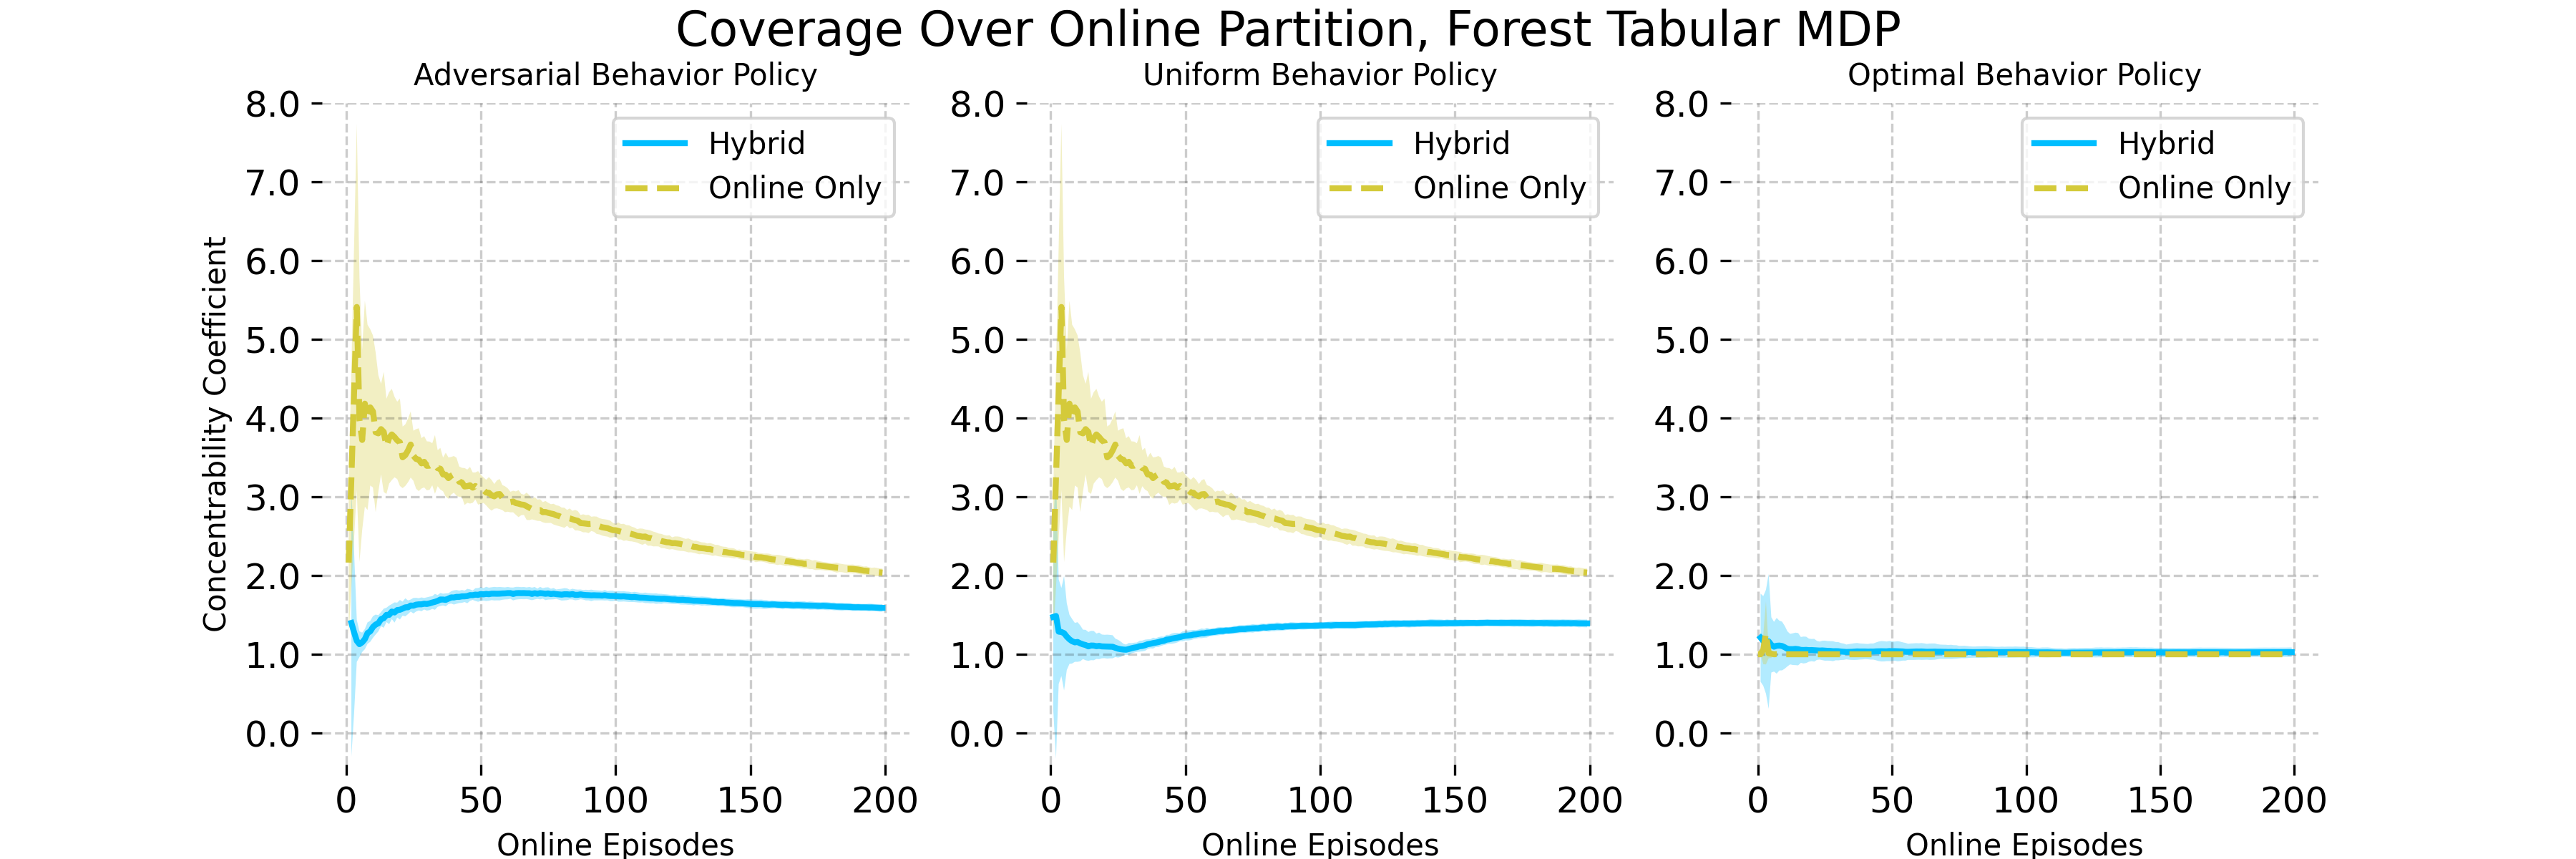
\includegraphics[width=0.48\textwidth]{figures/ch02/figs/cov_tabular_onpart.png}
    \hfill
    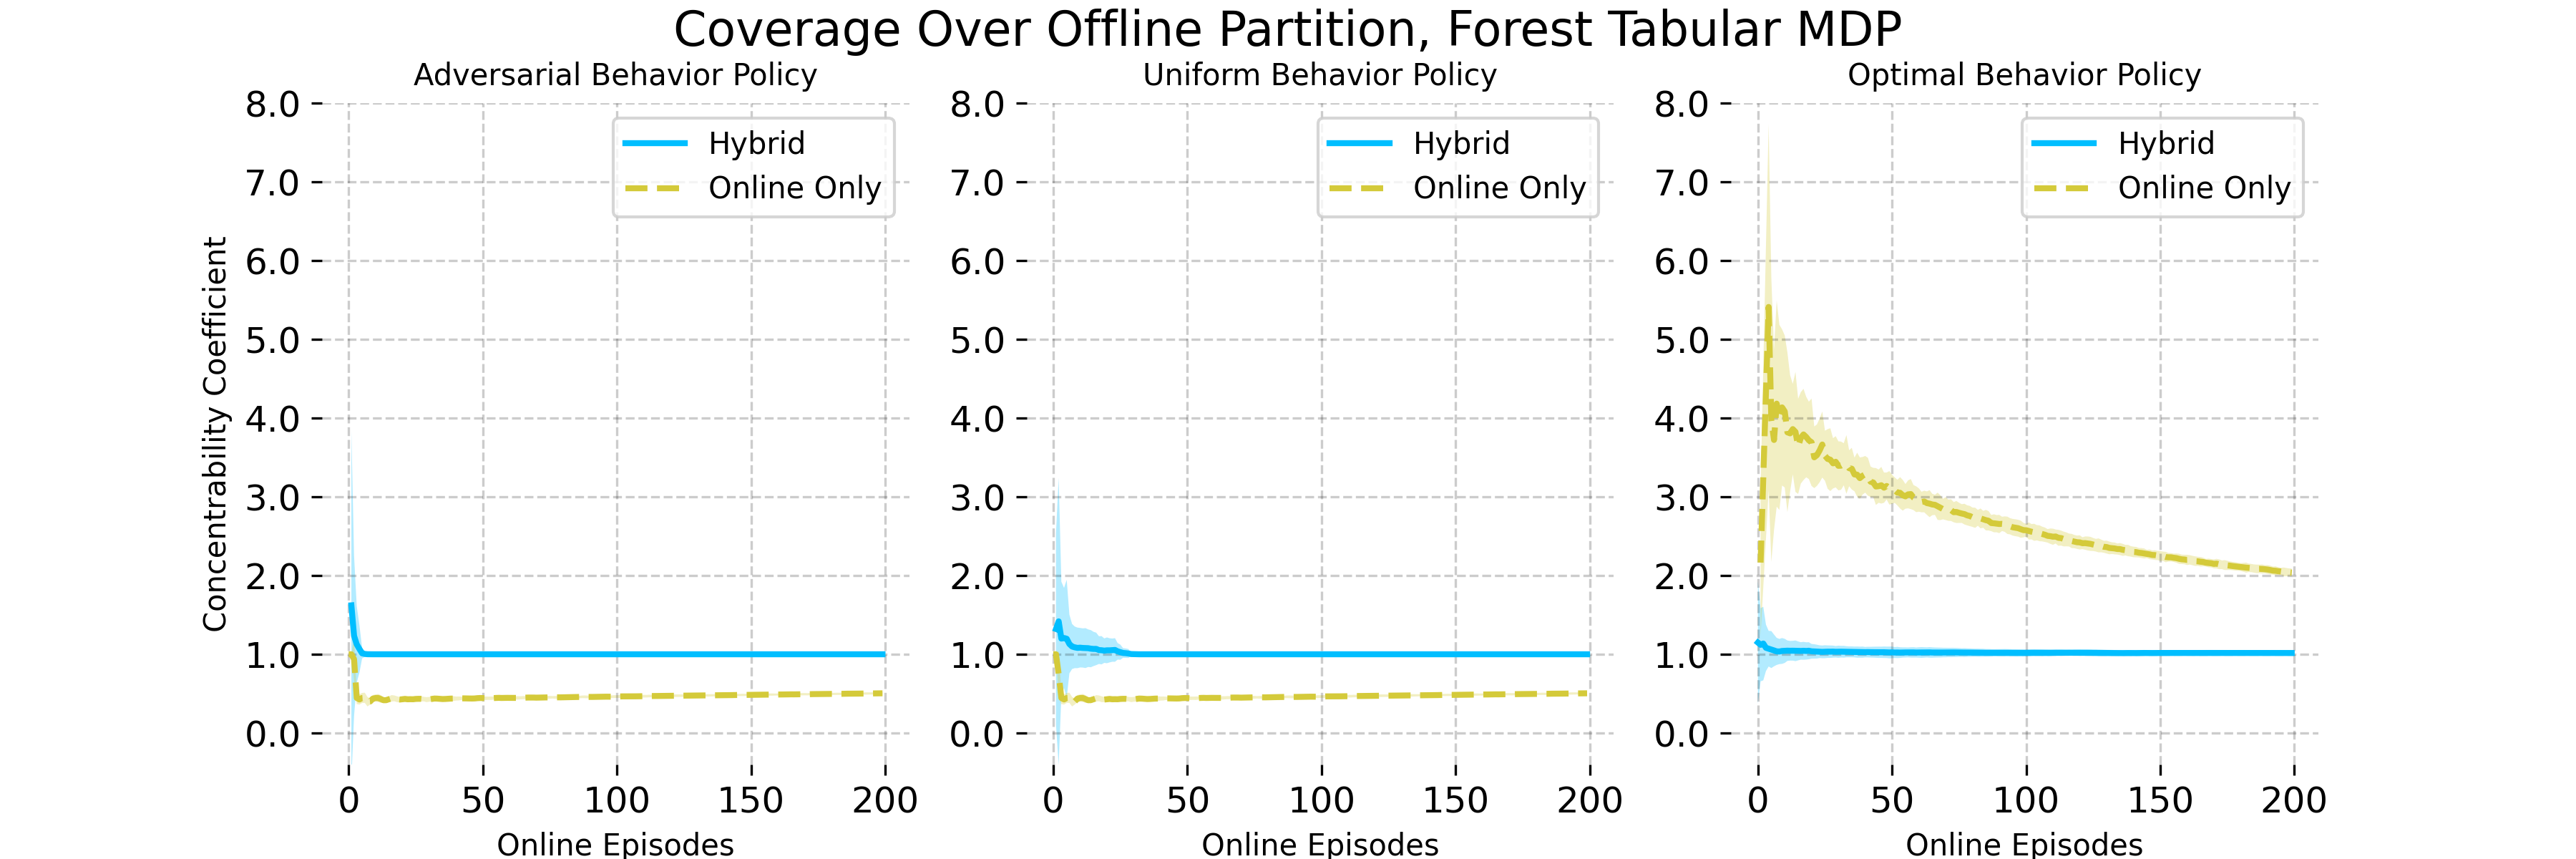
\includegraphics[width=0.48\textwidth]{figures/ch02/figs/cov_tabular_offpart.png}
    \caption{Coverage of online trajectories in the tabular forest management environment averaged over 30 trials (shaded bands indicate $\pm 1.96$ standard errors, where lower values correspond to better coverage). Left: online partition $\gX_{\on}$. Right: offline partition $\gX_{\off}$.}
    \label{fig:ch02-tabular-coverage}
\end{figure}

\subsection{Linear MDP: Scaled-Down Tetris}
We next consider a scaled-down Tetris environment with board width $6$, pieces of size at most $2 \times 2$, four rotation actions ($0^\circ, 90^\circ, 180^\circ, 270^\circ$), horizon $H = 40$, and reward equal to the negative increase in stack height above $2$. Following \citet{tan2024natural}, we project the $640$-dimensional one-hot state-action encoding onto the $60$-dimensional subspace spanned by the top $60$ eigenvectors of the offline covariance matrix estimated from $N_{\off} = 200$ uniform-policy trajectories, taking $\Phi_{\off}$ as the top $5$ eigenvectors and $\Phi_{\on}$ as the remaining $55$ eigenvectors. Figure~\ref{fig:ch02-linear-coverage} compares the full and partial all-policy concentrability coefficients of LSVI-UCB \citep{jin2020provably} with and without offline replay initialization over $N_{\on} = 100$ online episodes, confirming that offline initialization accelerates exploration across both the full space and the online subspace.

\begin{figure}[htbp]
    \centering
    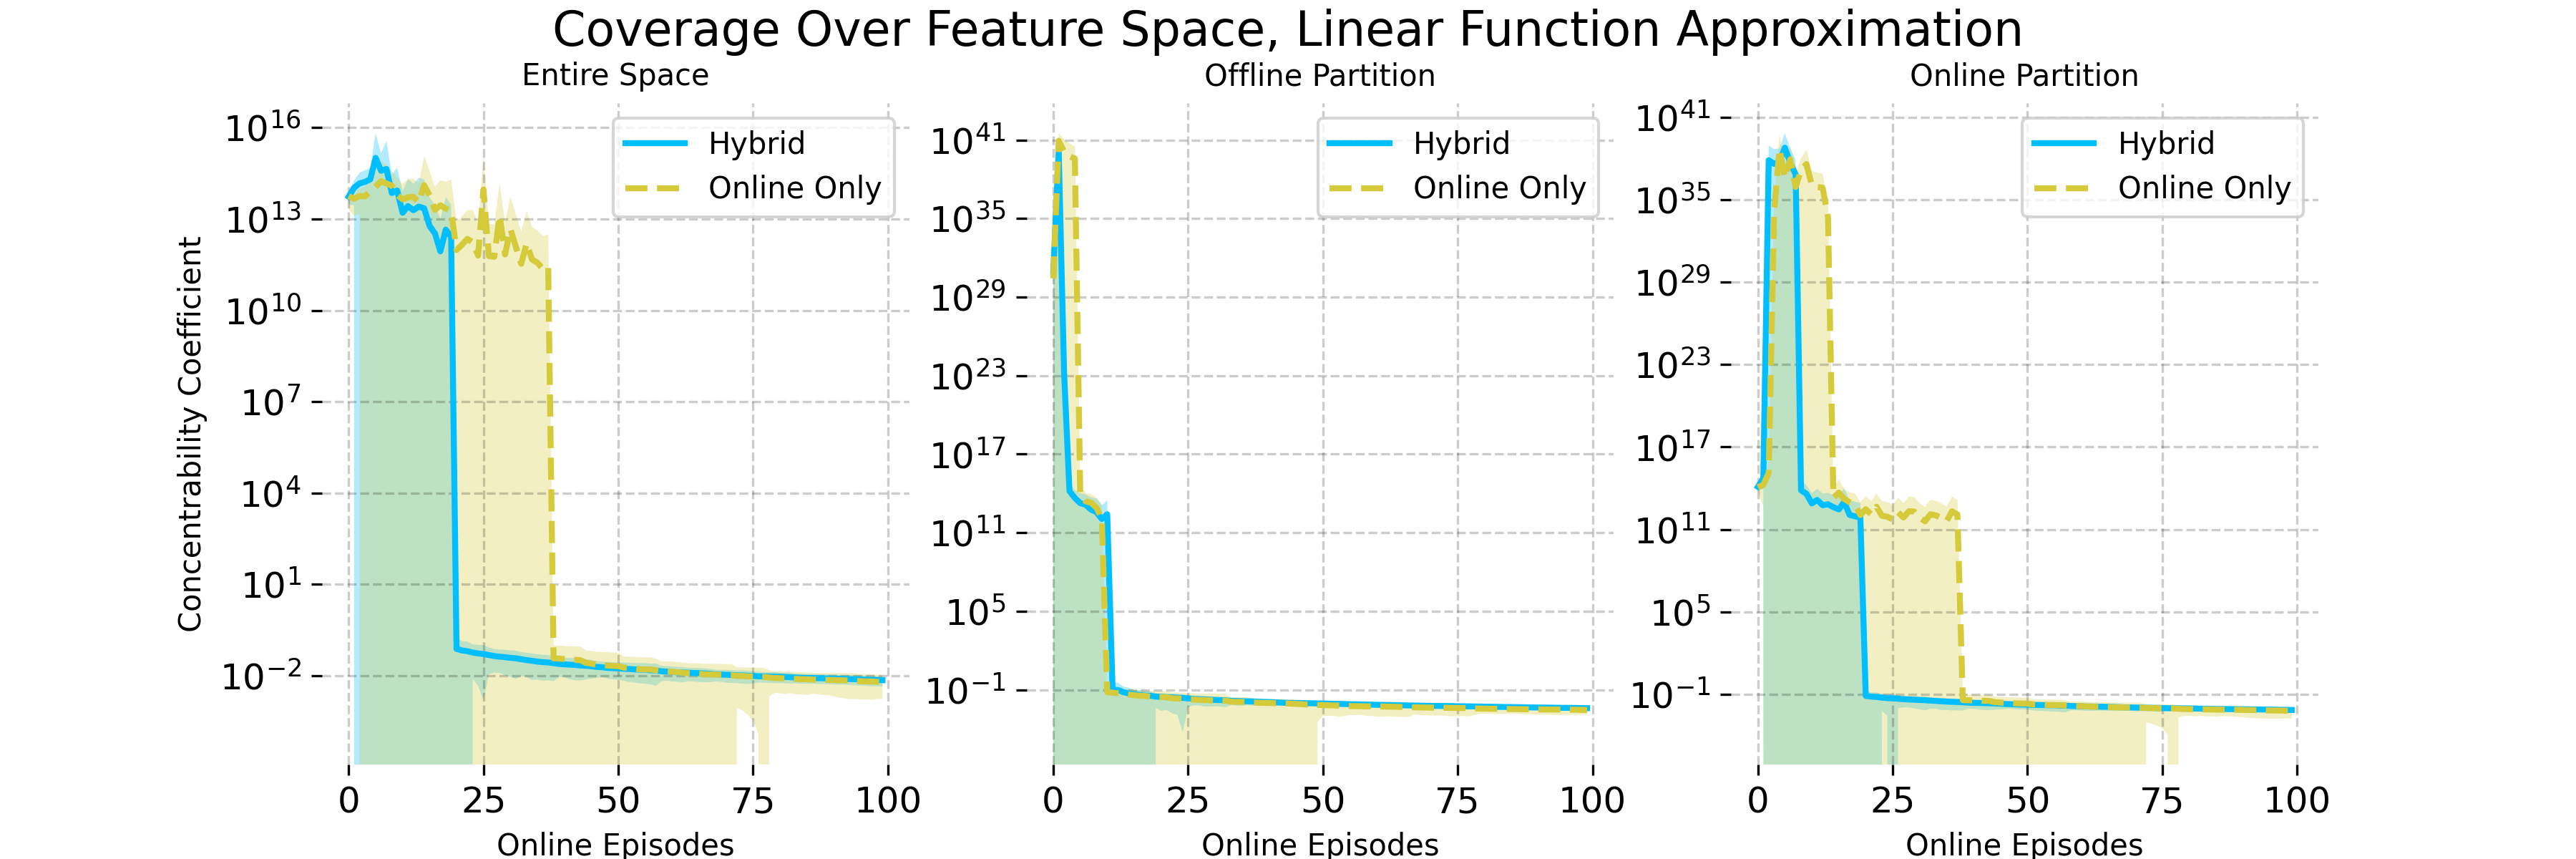
\includegraphics[width=0.65\textwidth]{figures/ch02/figs/cov_linear.png}
    \caption{Full and partial all-policy concentrability coefficients of online samples in the linear Tetris environment over 100 online episodes (mean over 30 trials $\pm 1.96$ standard errors, where lower is better).}
    \label{fig:ch02-linear-coverage}
\end{figure}

% =========================================================================
% PART 2: BREAKING SAMPLE SIZE BARRIERS IN LINEAR MDPS (Tan, Fan, Wei 2024)
% =========================================================================

\section{Breaking Sample Size Barriers in Linear MDPs}
\label{sec:ch02-lin-intro}

While \aigen{Algorithm~\ref{alg:ch02-alg1}} applies to any Bellman-complete function class, its specialization to $d$-dimensional linear MDPs in Proposition~\ref{prop:ch02-case_linear} yields a regret bound of $\tilde{\gO}(\sqrt{c_{\off}(\gX_{\off}) d H^5 N_{\on}^2 / N_{\off}} + \sqrt{d_{\on} d H^5 N_{\on}})$. In purely online linear MDPs, the minimax-optimal regret is $\tilde{\Theta}(\sqrt{d^2 H^3 T})$ \citep{zhou2021nearly, he2023nearly, hu2023nearlynot, agarwal2022voql}, and in purely offline linear MDPs, variance-weighted pessimistic value iteration achieves the minimax-optimal instance-dependent suboptimality bound $\tilde{\gO}(\sqrt{d}\sum_{h=1}^H \E_{\pi^\star}\|\phi(s_h, a_h)\|_{(\mSigma_{\off, h}^\star)^{-1}}) \leq \tilde{\gO}(\sqrt{C^\star d^2 H^4 / N_{\off}})$ \citep{xiong2023nearly}. Likewise, the reward-agnostic hybrid linear MDP algorithm of \citet{wagenmaker2023leveraging} attains a worst-case suboptimality bound of $\tilde{\gO}(\sqrt{d^2 H^7 / N})$. Thus, existing general or reward-agnostic hybrid bounds in linear MDPs lose factors of $H^2$ to $H^4$ relative to the optimal purely online and purely offline rates, as summarized in Tables~\ref{tab:ch02-prev-lit} and~\ref{tab:ch02-best-bounds}.

\begin{table}[htbp]
\centering
\resizebox{\linewidth}{!}{
\begin{tabular}{ccccc}
\toprule
Work & Function Class & Single-Policy Concentrability & Beats Pure Lower Bounds? & Guarantee \\
\midrule
\citet{song2023hybrid}, \citet{nakamoto2023calql} & General & Required & No & Regret \\
\citet{amortila2024harnessing} & General & Required & No & Regret \\
\aigen{Algorithm~\ref{alg:ch02-alg1}} \citep{tan2024natural} & General & Not Required & No ($H^5$ in linear) & Regret \\
\citet{wagenmaker2023leveraging} & Linear & Not Required & No ($H^7$ worst-case) & PAC \\
\citet{li2023reward} & Tabular & Not Required & Yes & PAC \\
Algorithms~\ref{alg:ch02-alg2} and~\ref{alg:ch02-alg3} \citep{tan2024hybrid} & Linear & Not Required & Yes & PAC, Regret \\
\bottomrule
\end{tabular}
}
\caption{Comparison of hybrid RL approaches by function approximation class, coverage assumptions, and whether they improve upon purely offline or purely online minimax lower bounds.}
\label{tab:ch02-prev-lit}
\end{table}

\begin{table}[htbp]
\centering
\resizebox{\linewidth}{!}{
\begin{tabular}{c|c|c}
\toprule
Setting & Upper Bound & Lower Bound \\
\midrule
Offline Linear MDP (PAC Error) & $\sqrt{d}\sum_{h=1}^H \E_{\pi^\star}\|\phi(s_h, a_h)\|_{(\mSigma_{\off, h}^\star)^{-1}} \leq \sqrt{C^\star d^2 H^4 / N_{\off}}$ \citep{xiong2023nearly} & $\sqrt{C^\star d^2 H^2 / N_{\off}}$ \citep{xiong2023nearly} \\
Online Linear MDP (Regret) & $\sqrt{d^2 H^3 T}$ \citep{he2023nearly} & $\sqrt{d^2 H^3 T}$ \citep{zhou2021nearly} \\
\midrule
Hybrid Paradigm & \multicolumn{2}{c}{Guarantee} \\
\midrule
Online-to-Offline (PAC Error) & \multicolumn{2}{c}{$\sqrt{d^2 H^7 / N}$ \citep{wagenmaker2023leveraging}} \\
& \multicolumn{2}{c}{$\sqrt{c_{\off}(\gX_{\off}) d H^3 \min\{c_{\off}(\gX_{\off}), H\}/N_{\off}} + \sqrt{d_{\on} d H^3 \min\{d_{\on}, H\}/N_{\on}}$ (\textbf{\aigen{Algorithm~\ref{alg:ch02-alg2}}})} \\
\midrule
Offline-to-Online (Regret) & \multicolumn{2}{c}{$C^\star \sqrt{d^2 H^6 N_{\on}}$ \citep{song2023hybrid, nakamoto2023calql}} \\
& \multicolumn{2}{c}{$\sqrt{(C^\star + c_{\on}(\gX)) d^3 H^6 N_{\on}}$ \citep{amortila2024harnessing}} \\
& \multicolumn{2}{c}{$\sqrt{c_{\off}(\gX_{\off}) d H^5 N_{\on}^2 / N_{\off}} + \sqrt{d_{\on} d H^5 N_{\on}}$ (\textbf{\aigen{Algorithm~\ref{alg:ch02-alg1}}})} \\
& \multicolumn{2}{c}{$\sqrt{c_{\off}(\gX_{\off})^2 d H^3 N_{\on}^2 / N_{\off}} + \sqrt{d_{\on} d H^3 N_{\on}}$ (\textbf{\aigen{Algorithm~\ref{alg:ch02-alg3}}})} \\
\bottomrule
\end{tabular}
}
\caption{Comparison of PAC error and cumulative regret bounds for offline, online, and hybrid RL in $d$-dimensional episodic linear MDPs with horizon $H$.}
\label{tab:ch02-best-bounds}
\end{table}

In the remainder of this chapter, we study both major paradigms of hybrid RL in linear MDPs:
\begin{itemize}
    \item \textbf{Online-to-offline PAC learning (Section~\ref{sec:ch02-lin-pac}):} When the goal is to output a single deterministic policy $\widehat{\pi}$ for deployment after exploration, randomizing over an online policy history (as in regret-to-PAC conversion) is often undesirable in safety-critical applications. Moreover, reward-agnostic online exploration produces a combined dataset that can be reused across multiple downstream reward functions. \aigen{Algorithm~\ref{alg:ch02-alg2}} combines reward-agnostic covariate collection \citep{wagenmaker2023instancedependent} with variance-weighted pessimistic value iteration \citep{xiong2023nearly} to achieve an error bound of $\tilde{\gO}(\sqrt{c_{\off}(\gX_{\off}) d H^3 \min\{c_{\off}(\gX_{\off}), H\} / N_{\off}} + \sqrt{d_{\on} d H^3 \min\{d_{\on}, H\} / N_{\on}})$.
    \item \textbf{Offline-to-online regret minimization (Section~\ref{sec:ch02-lin-regret}):} When the agent must maintain high reward throughout online interaction, \aigen{Algorithm~\ref{alg:ch02-alg3}} warm-starts variance-weighted optimistic value iteration \citep{he2023nearly} with offline parameter and variance estimates, achieving $\Reg(N_{\on}) = \tilde{\gO}(\inf_{\gX_{\off}, \gX_{\on}}\{\sqrt{c_{\off}(\gX_{\off})^2 d H^3 N_{\on}^2 / N_{\off}} + \sqrt{d_{\on} d H^3 N_{\on}}\})$ without knowing the partition.
\end{itemize}

\paragraph{Additional Linear MDP Notation.}
In a linear MDP satisfying Definition~\ref{defn:ch02-linear_MDP}, write $\phi_{n,h} = \phi(s_h^{(n)}, a_h^{(n)})$ for the feature vector observed at episode $n$ and step $h$. Let $\boldsymbol{\Lambda}_h = \sum_{n=1}^N \phi_{n,h}\phi_{n,h}^{\top}+\lambda\mathbf{I}$ and $\boldsymbol{\Lambda}_{\off, h} = \sum_{n=1}^{N_{\off}} \phi_{n,h}\phi_{n,h}^{\top}+\lambda\mathbf{I}$ denote the unweighted ridge covariance matrices of the combined dataset and the offline dataset, respectively, and let $\boldsymbol{\Omega}$ denote the set of population feature covariance matrices induced by policies in $\Pi$. We consider two variance-weighted covariance matrices:
\begin{equation}
    \boldsymbol{\Sigma}_{h}^{\star} = \sum_{n=1}^N \frac{\phi_{n,h}\phi_{n,h}^{\top}}{\left[\mathbb{V}_h V_{h+1}^\star\right]\!\left(s_h^{(n)}, a_h^{(n)}\right)}+\lambda\mathbf{I}, \qquad
    \boldsymbol{\Sigma}_{t,h} = \sum_{n=1}^{N_{\off}+t-1} \bar{\sigma}_{n,h}^{-2}\phi_{n,h}\phi_{n,h}^{\top}+\lambda\mathbf{I},
\end{equation}
where $[\mathbb{V}_h V_{h+1}^\star](s, a) = \max\{1, [\operatorname{Var}_h V_{h+1}^\star](s, a)\}$ is the truncated conditional variance of the optimal value function and $\bar{\sigma}_{n,h}^{2}$ is the variance estimator of \citet{he2023nearly}. For any partition $\gX_{\on} \cup \gX_{\off} = \gX$ with projected subspaces $\Phi_{\off}$ (dimension $d_{\off}$, projector $\gP_{\off}$) and $\Phi_{\on}$ (dimension $d_{\on}$, projector $\gP_{\on}$), we write the linear-MDP partial offline concentrability and partial online coverability coefficients as
\begin{align}
    c_{\off}(\gX_{\off}) &\coloneqq \max_{h \in [H]} \frac{1}{\lambda_{d_{\off}}\!\left(\E_{\mu_h}[(\gP_{\off}\phi_h)(\gP_{\off}\phi_h)^{\top}]\right)}, \label{eq:ch02-c_off} \\
    c_{\on}(\gX_{\on}) &\coloneqq \inf_{\pi \in \Pi} \max_{h \in [H]} \frac{1}{\lambda_{d_{\on}}\!\left(\E_{d^\pi_h}[(\gP_{\on}\phi_h)(\gP_{\on}\phi_h)^{\top}]\right)}. \label{eq:ch02-c_on}
\end{align}

\section{Online-to-Offline PAC Learning in Linear MDPs}
\label{sec:ch02-lin-pac}

Given the offline dataset $\gD_{\off}$ with covariance matrices $\boldsymbol{\Lambda}_{\off, h}$, \aigen{Algorithm~\ref{alg:ch02-alg2}} first runs the reward-agnostic covariate-collection subroutine of \citet{wagenmaker2023instancedependent} (stated in full in Appendix~\ref{app:ch02-unabridged}) to collect online trajectories until the maximum leverage score $\max_{\phi_h \in \Phi} \phi_h^\top (\boldsymbol{\Lambda}_h + \lambda \mathbf{I} + \boldsymbol{\Lambda}_{\off, h})^{-1}\phi_h$ falls below a target tolerance $\tau$. It then runs variance-weighted pessimistic value iteration \citep{xiong2023nearly} on the combined dataset $\gD_{\off} \cup \gD_{\on}$ to output a deterministic policy $\widehat{\pi}$.

\begin{algorithm}[htbp]
    \caption{Online-to-Offline Hybrid RL via Reward-Agnostic Exploration and Pessimistic Planning}
    \label{alg:ch02-alg2}
    \begin{algorithmic}[1]
        \State {\bfseries Input:} Offline dataset $\gD_{\off}$, sample sizes $N_{\on}$, $N_{\off}$, feature maps $\phi_h$, exploration tolerance parameter $\tau > 0$.
        \State {\bfseries Initialize:} $\gD_h^{(0)}\leftarrow \emptyset$ for all $h \in [H]$, $\lambda = 1/H^2$, $\beta_2 = \tilde{O}(\sqrt{d})$.
        \For{step $h=1,\dots,H$}
            \State Run reward-agnostic covariate collection \citep{wagenmaker2023instancedependent} to collect online covariates $\boldsymbol{\Lambda}_{h}$ until
            \begin{equation*}
                \max_{\phi_h \in \Phi} \phi_h^{\top}(\boldsymbol{\Lambda}_{h} + \lambda \mathbf{I} + \boldsymbol{\Lambda}_{\off,h})^{-1}\phi_h \leq \tau.
            \end{equation*}
        \EndFor
        \State {\bfseries Output:} Policy $\widehat{\pi}$ obtained by running variance-weighted pessimistic value iteration \citep{xiong2023nearly} with parameters $\lambda, \beta_2$ on the combined dataset $\gD_{\off} \cup \{\gD^{(N_{\on})}_h\}_{h \in [H]}$.
    \end{algorithmic}
\end{algorithm}

To guarantee that the reward-agnostic exploration phase terminates, we impose a full-rank projected covariate condition analogous to that of \citet{wagenmaker2023leveraging}. This assumption is used only for \aigen{Algorithm~\ref{alg:ch02-alg2}}.

\begin{aspt}[Full-Rank Projected Covariates]
\label{aspt:ch02-full-rank-proj-covariates}
For any partition $\gX_{\on} \cup \gX_{\off} = \gX$, we have $c_{\on}(\gX_{\on}) < \infty$, or equivalently,
\begin{equation}
    \sup_{\pi \in \Pi} \min_{h \in [H]} \lambda_{d_{\on}}\!\left(\E_{d^\pi_h}[(\gP_{\on}\phi_h)(\gP_{\on}\phi_h)^{\top}]\right) = \lambda^\star_{d_{\on}} > 0.
\end{equation}
\end{aspt}

By applying the Kiefer--Wolfowitz theorem \citep{lattimore2020learning} on the $d_{\on}$-dimensional projected feature space $\Phi_{\on}$ and an eigenspace truncation on $\Phi_{\off}$, Lemma~\ref{lem:ch02-cov-linear} bounds the partial coverability and concentrability coefficients by the subspace dimensions.

\begin{lem}[Bounded Partial Coverability in Linear MDPs]
\label{lem:ch02-cov-linear}
For any partition $\gX_{\off}, \gX_{\on}$ of $\gX$, we have $c_{\on}(\gX_{\on}) \leq d_{\on}$. Moreover, there always exists at least one partition such that $c_{\off}(\gX_{\off}) = \gO(d)$.
\end{lem}

Let $\alpha_{\off} \coloneqq N_{\off}/N$, $\alpha_{\on} \coloneqq N_{\on}/N$, and define the minimal online sample complexity required to achieve tolerance $\tau$ by
\begin{equation}
    N^\star(\tau) \coloneqq \min \left\{ N \in \sN : \inf_{\boldsymbol{\Lambda} \in \boldsymbol{\Omega}} \max_{\boldsymbol{\phi} \in \Phi} \boldsymbol{\phi}^{\top}\!\left(N(\boldsymbol{\Lambda}+\bar{\lambda} \mathbf{I})+\boldsymbol{\Lambda}_{\mathrm{off}}\right)^{-1} \boldsymbol{\phi} \leq \tau \right\}.
\end{equation}
Theorem~\ref{thm:ch02-hybridoffline} establishes both an instance-dependent suboptimality bound and a worst-case partitioned suboptimality bound for \aigen{Algorithm~\ref{alg:ch02-alg2}}, with the full proof is given in Appendix~\ref{app:ch02-hybridoffline}.

\begin{thm}[PAC Suboptimality Bound for \aigen{Algorithm~\ref{alg:ch02-alg2}}]
\label{thm:ch02-hybridoffline}
Suppose Assumption~\ref{aspt:ch02-full-rank-proj-covariates} holds. For every $\delta \in (0,1)$ and any partition $\gX_{\off}, \gX_{\on}$, when $\tau \leq \tilde{\gO}(\max\{d_{\on}/N_{\on}, c_{\off}(\gX_{\off})/N_{\off}\})$ and $N \geq \max\{\alpha_{\on}^{4} d_{\on}^{-4}, \alpha_{\off}^{4} c_{\off}(\gX_{\off})^{-4}\}\max\{N^\star(\tau), \operatorname{poly}(d, H, c_{\off}(\gX_{\off}), \log(1/\delta))\}$, \aigen{Algorithm~\ref{alg:ch02-alg2}} achieves with probability at least $1-\delta$:
\begin{align}
    V_1^\star(s)-V_1^{\widehat{\pi}}(s) &\lesssim \sqrt{d}\sum_{h=1}^H \E_{\pi^\star}\|\phi(s_h, a_h)\|_{(\boldsymbol{\Sigma}_{\off,h}^{\star}+ \boldsymbol{\Sigma}_{\on,h}^\star)^{-1}}\leq \sqrt{d}\sum_{h=1}^H \E_{\pi^\star}\|\phi(s_h, a_h)\|_{(\boldsymbol{\Sigma}_{\off,h}^{\star})^{-1}}, \label{eqn:ch02-rappel-res1}\\
    V_1^\star(s)-V_1^{\widehat{\pi}}(s) &\lesssim \min\left\{\sqrt{\frac{c_{\off}(\gX_{\off})dH^{4}}{N_{\off}}} + \sqrt{\frac{d_{\on}dH^{4}}{N_{\on}}},\; \sqrt{\frac{c_{\off}(\gX_{\off})^2dH^3}{N_{\off}\alpha_{\off}}} + \sqrt{\frac{d_{\on}^2dH^3}{N_{\on}\alpha_{\on}}}\right\}. \label{eqn:ch02-rappel-res2}
\end{align}
\end{thm}

When specialized to tabular MDPs with one-hot features $\phi(s,a) = \ve_{s,a} \in \sR^{S A}$, where $\pi^\star$ is deterministic, Theorem~\ref{thm:ch02-hybridoffline} yields an $H^3$ horizon dependence without the extra factor of $c_{\off}(\gX_{\off})$ or $d_{\on}$ (proof in Appendix~\ref{app:ch02-proof-cor-rappel-tab}).

\begin{cor}[Tabular Specialization of \aigen{Algorithm~\ref{alg:ch02-alg2}}]
\label{cor:ch02-rappel-tabular}
In a tabular MDP, for every $\delta\in (0,1)$, with probability at least $1-\delta$, \aigen{Algorithm~\ref{alg:ch02-alg2}} satisfies
\begin{equation}
    V_1^{\star}(s) - V_1^{\widehat{\pi}}(s) \lesssim \sqrt{H^3 S^2 A}\left(\sqrt{\frac{c_{\off}(\gX_{\off})}{N_{\off}}} + \sqrt{\frac{d_{\on}}{N_{\on}}}\right).
\end{equation}
\end{cor}

\paragraph{Proof Sketch for Theorem~\ref{thm:ch02-hybridoffline}.}
Equation~\eqref{eqn:ch02-rappel-res1} follows from invoking the instance-dependent suboptimality guarantee of \citet[Theorem 2]{xiong2023nearly} on the combined dataset $\gD_{\off} \cup \gD_{\on}$ and noting that $\mSigma^\star_h = \mSigma^\star_{\off, h} + \mSigma^\star_{\on, h} \succeq \mSigma^\star_{\off, h}$. To obtain Equation~\eqref{eqn:ch02-rappel-res2}, we decompose the expectation under $\pi^\star$ across $\Phi_{\on}$ and $\Phi_{\off}$:
\begin{equation}
    V_1^\star(s)-V_1^{\widehat{\pi}}(s) \lesssim \sqrt{d} \sum_{h=1}^H \max_{\phi_h \in \Phi_{\on}} \sqrt{\phi_h^{\top}(\boldsymbol{\Sigma}_h^{\star})^{-1}\phi_h} + \sqrt{d} \sum_{h=1}^H  \max_{\phi_h \in \Phi_{\off}}\sqrt{ \phi_h^{\top}(\boldsymbol{\Sigma}_h^{\star})^{-1}\phi_h}.
\end{equation}
Using $(\mSigma^\star_h)^{-1} \preceq H^2 \mLambda_h^{-1}$ together with Lemma~\ref{lem:ch02-cov-linear} and the stopping condition $\max_{\phi_h \in \Phi} \phi_h^\top \mLambda_h^{-1} \phi_h \lesssim \max\{c_{\off}(\gX_{\off})/N_{\off}, d_{\on}/N_{\on}\}$ immediately gives the first bound $\sqrt{c_{\off}(\gX_{\off}) d H^4 / N_{\off}} + \sqrt{d_{\on} d H^4 / N_{\on}}$. To sharpen the horizon dependence from $H^4$ to $H^3$, we observe that by the total variance lemma \citep[Lemma C.5]{jin2018q}, the empirical average over $(n, h)$ of $[\mathbb{V}_h V^\star_{h+1}](s_h^{(n)}, a_h^{(n)})$ is $\tilde{\gO}(H)$ rather than $H^2$. In Lemma~\ref{lem:ch02-total-variance-concentration}, we truncate the high-variance trajectories at each step $h$ where $[\mathbb{V}_h V^\star_{h+1}] \geq C_h \bar{\sigma}_h$, bound their cardinality via Markov's inequality, and choose $C_h$ so that the remaining low-variance trajectories preserve at least half of the minimum eigenvalue of $\mLambda_h$, yielding the second bound in Equation~\eqref{eqn:ch02-rappel-res2}.

\section{Offline-to-Online Regret Minimization in Linear MDPs}
\label{sec:ch02-lin-regret}

When the agent must minimize cumulative regret during online interaction, reward-agnostic exploration is unsuitable. \aigen{Algorithm~\ref{alg:ch02-alg3}} warm-starts variance-weighted optimistic value iteration \citep{he2023nearly} by computing initial optimistic and pessimistic weight vectors $\widehat{\vw}_{1,h}, \widecheck{\vw}_{1,h}$, action-value functions $Q_{1,h}, \widecheck{Q}_{1,h}$, and variance weights $\bar{\sigma}_{n,h}^2$ on the $N_{\off}$ offline episodes, and initializing the precision matrix as $\mSigma_{1,h} = \sum_{n=1}^{N_{\off}} \bar{\sigma}_{n,h}^{-2}\phi_{n,h}\phi_{n,h}^\top + \lambda \mathbf{I}$. The unabridged pseudocode is given in Appendix~\ref{app:ch02-unabridged}.

\begin{algorithm}[htbp]
    \caption{Offline-to-Online Hybrid RL via Variance-Weighted Optimistic Value Iteration}
    \label{alg:ch02-alg3}
    \begin{algorithmic}[1]
        \State {\bfseries Input:} Offline dataset $\gD_{\off}$, sample sizes $N_{\on}$, $N_{\off}$, feature maps $\phi_h$, regularization $\lambda>0$, confidence radii $\beta, \bar\beta, \tilde\beta$, determinant update index $t_{\text{last}}=0$.
        \State {\bfseries Initialize:} For each $h \in [H]$, estimate $\widehat{\mathbf{w}}_{1, h}, \widecheck{\mathbf{w}}_{1, h}, Q_{1,h}, \widecheck{Q}_{1,h}, \sigma_{n,h}, \bar{\sigma}_{n,h}$ from $\gD_{\off}$, and set
        \begin{equation*}
            \boldsymbol{\Sigma}_{0, h}=\boldsymbol{\Sigma}_{1, h}=\boldsymbol{\Sigma}_{\off, h} + \lambda\mathbf{I} = \sum_{n=1}^{N_{\off}}\bar{\sigma}_{n,h}^{-2}\phi_{n,h}\phi_{n,h}^{\top}+\lambda\mathbf{I}.
        \end{equation*}
        \For{episode $t=1,\dots,T$}
            \State Update optimistic and pessimistic weights $\widehat{\mathbf{w}}_{t, h}, \widecheck{\mathbf{w}}_{t, h}$ for all $h \in [H]$.
            \If{there exists $h^{\prime} \in[H]$ such that $\operatorname{det}\!\left(\boldsymbol{\Sigma}_{t, h^{\prime}}\right) \geq 2 \operatorname{det}\!\left(\boldsymbol{\Sigma}_{t_{\text {last }}, h^{\prime}}\right)$}
                \State Update optimistic and pessimistic action-value functions $Q_{t, h}(s, a), \widecheck{Q}_{t, h}(s, a)$ for all $h \in [H]$ and set $t_{\text {last }}=t$.
            \EndIf
            \For{step $h=1,\dots,H$}
                \State Execute action $a_h^{(t)} \leftarrow \argmax_{a \in \gA} Q_{t,h}(s_h^{(t)}, a)$ and observe $r_h^{(t)}, s_{h+1}^{(t)}$.
                \State Compute variance estimate $\sigma_{t, h}$, set ${\bar{\sigma}}_{t, h} \leftarrow \max \{\sigma_{t, h}, \sqrt{H}, 2 d^3 H^2\|\boldsymbol{\phi}(s_h^{(t)}, a_h^{(t)})\|_{\boldsymbol{\Sigma}_{t, h}^{-1}}^{1 / 2}\}$, and update $\boldsymbol{\Sigma}_{t+1, h} \leftarrow \boldsymbol{\Sigma}_{t, h} + \bar{\sigma}_{t, h}^{-2}\phi_{t,h}\phi_{t,h}^\top$.
            \EndFor
        \EndFor
        \State {\bfseries Output:} Greedy policy $\widehat{\pi} = \pi^{Q_{T,h}}$ (or uniform mixture $\operatorname{Unif}(\pi^{Q_{1,h}},\dots,\pi^{Q_{T,h}})$ for PAC conversion).
    \end{algorithmic}
\end{algorithm}

Theorem~\ref{thm:ch02-hybridonline} establishes the cumulative regret bound of \aigen{Algorithm~\ref{alg:ch02-alg3}}, with the full proof is given in Appendix~\ref{app:ch02-hybridonline}.

\begin{thm}[Regret Bound for \aigen{Algorithm~\ref{alg:ch02-alg3}}]
\label{thm:ch02-hybridonline}
For any $\delta \in (0,1)$, if $N_{\on}, N_{\off} = \tilde{\Omega}(d^{13}H^{14})$, then with probability at least $1-\delta$, \aigen{Algorithm~\ref{alg:ch02-alg3}} satisfies
\begin{equation}
    \Reg(N_{\on}) \lesssim \inf_{\gX_{\off}, \gX_{\on}}\left\{\sqrt{c_{\off}(\gX_{\off})^{2}dH^3\frac{N_{\on}^2}{N_{\off}}} + \sqrt{d_{\on}d H^3N_{\on}}\right\}.
\end{equation}
\end{thm}

\begin{cor}[Regret-to-PAC Conversion for \aigen{Algorithm~\ref{alg:ch02-alg3}}]
\label{cor:ch02-hyrule-pac}
Under the conditions of Theorem~\ref{thm:ch02-hybridonline}, the uniform mixture policy $\widehat{\pi} = \operatorname{Unif}(\pi^{Q_{1,h}},\dots,\pi^{Q_{T,h}})$ output by \aigen{Algorithm~\ref{alg:ch02-alg3}} satisfies, with probability at least $1-\delta$,
\begin{equation}
    V_1^\star(s)-V_1^{\widehat{\pi}}(s)\lesssim \inf_{\gX_{\off}, \gX_{\on}}\left\{\sqrt{\frac{c_{\off}(\gX_{\off})^2dH^3}{N_{\off}}} + \sqrt{\frac{d_{\on}d H^3}{N_{\on}}}\right\}.
\end{equation}
\end{cor}

\paragraph{Comparison and Proof Sketch for Theorem~\ref{thm:ch02-hybridonline}.}
Like \aigen{Algorithm~\ref{alg:ch02-alg1}}, \aigen{Algorithm~\ref{alg:ch02-alg3}} requires no knowledge of the partition $(\gX_{\off}, \gX_{\on})$ and automatically adapts to the infimum over all partitions. Taking $\gX_{\on} = \gX$ and $\gX_{\off} = \emptyset$ immediately recovers the minimax-optimal purely online regret bound $\tilde{\gO}(\sqrt{d^2 H^3 N_{\on}})$ of \citet{he2023nearly}, while in the offline-abundant regime $N_{\off} \gg N_{\on}$ the online regret scales as $\tilde{\gO}(\sqrt{d_{\on} d H^3 N_{\on}})$, breaking the $\Omega(\sqrt{d^2 H^3 N_{\on}})$ purely online lower bound whenever the offline dataset covers a subspace of dimension $d_{\off} = d - d_{\on} \geq 1$. Compared to Proposition~\ref{prop:ch02-case_linear} for \aigen{Algorithm~\ref{alg:ch02-alg1}}, Theorem~\ref{thm:ch02-hybridonline} sharpens the horizon dependence from $H^5$ to $H^3$.

To prove Theorem~\ref{thm:ch02-hybridonline}, we decompose the exploration bonuses across $\gX_{\off}$ and $\gX_{\on}$:
\begin{equation}
    \Reg(T) \lesssim \sqrt{H^3 T \log(H/\delta)} + \beta \sum_{t=1}^T \sum_{h=1}^H \|\boldsymbol{\Sigma}_{t,h}^{-1/2}\phi_h(s_h^{(t)},a_h^{(t)})\mathbbm{1}_{\gX_{\off}}\|_2 + \beta \sum_{t=1}^T \sum_{h=1}^H \|\boldsymbol{\Sigma}_{t,h}^{-1/2}\phi_h(s_h^{(t)},a_h^{(t)})\mathbbm{1}_{\gX_{\on}}\|_2.
\end{equation}
On the offline partition $\gX_{\off}$, since $\mSigma_{t,h} \succeq \mSigma_{\off, h} + \lambda \mathbf{I}$, Lemma~\ref{lem:ch02-hybridoffline-sumbonuses} bounds the sum of bonuses by $\sum_{h=1}^H \sqrt{d (N_{\on}^2 / N_{\off})} \sqrt{\max_{\phi_h \in \Phi_{\off}} \phi_h^\top \bar{\mSigma}_{\off, h}^{-1} \phi_h}$. Controlling $\bar{\mSigma}_{\off, h}^{-1}$ with $H^3$ rather than $H^4$ or $H^8$ requires ruling out the trajectories $n \in \gI_2 \subset [N_{\off}]$ where the leverage-score floor $4 d^6 H^4 \|\phi_{n,h}\|_{\mSigma_{n,h}^{-1}}$ dominates $\bar{\sigma}_{n,h}^2$. Using the elliptical potential lemma, we show $|\gI_2| \lesssim d^{13} H^5 \log(1 + N/d) = \tilde{o}(N_{\off})$, and then apply the variance-truncation bound in Lemma~\ref{lem:ch02-total-variance-concentration} together with the total variance bound $\frac{1}{N_{\off}}\sum_{n,h} \sigma_{n,h}^2 = \tilde{\gO}(H^2)$ on the remaining good trajectories $\gI_1$ in Lemma~\ref{lem:ch02-hybridoffline-concentrability}. On the online partition $\gX_{\on}$, we establish a projected subspace elliptical potential bound in Lemma~\ref{lem:ch02-zhou2022-B1-modified} using thin-SVD projection $U_{\on} U_{\on}^\top$ inside the matrix inverse (Lemma~\ref{lem:ch02-hole-digging}), reducing the dimension factor in the variance-weighted bonus sum from $d$ to $d_{\on}$ in Lemma~\ref{lem:ch02-hybridonline-sumbonuses-xon}.

\section{Numerical Experiments in Linear MDPs}
\label{sec:ch02-lin-sims}

We evaluate Algorithms~\ref{alg:ch02-alg2} and~\ref{alg:ch02-alg3} on the scaled-down linear Tetris environment described in Section~\ref{sec:ch02-gfa-sims} ($60$-dimensional SVD feature representation, $N_{\off} = 200$ offline trajectories).

\begin{figure}[htbp]
    \centering
    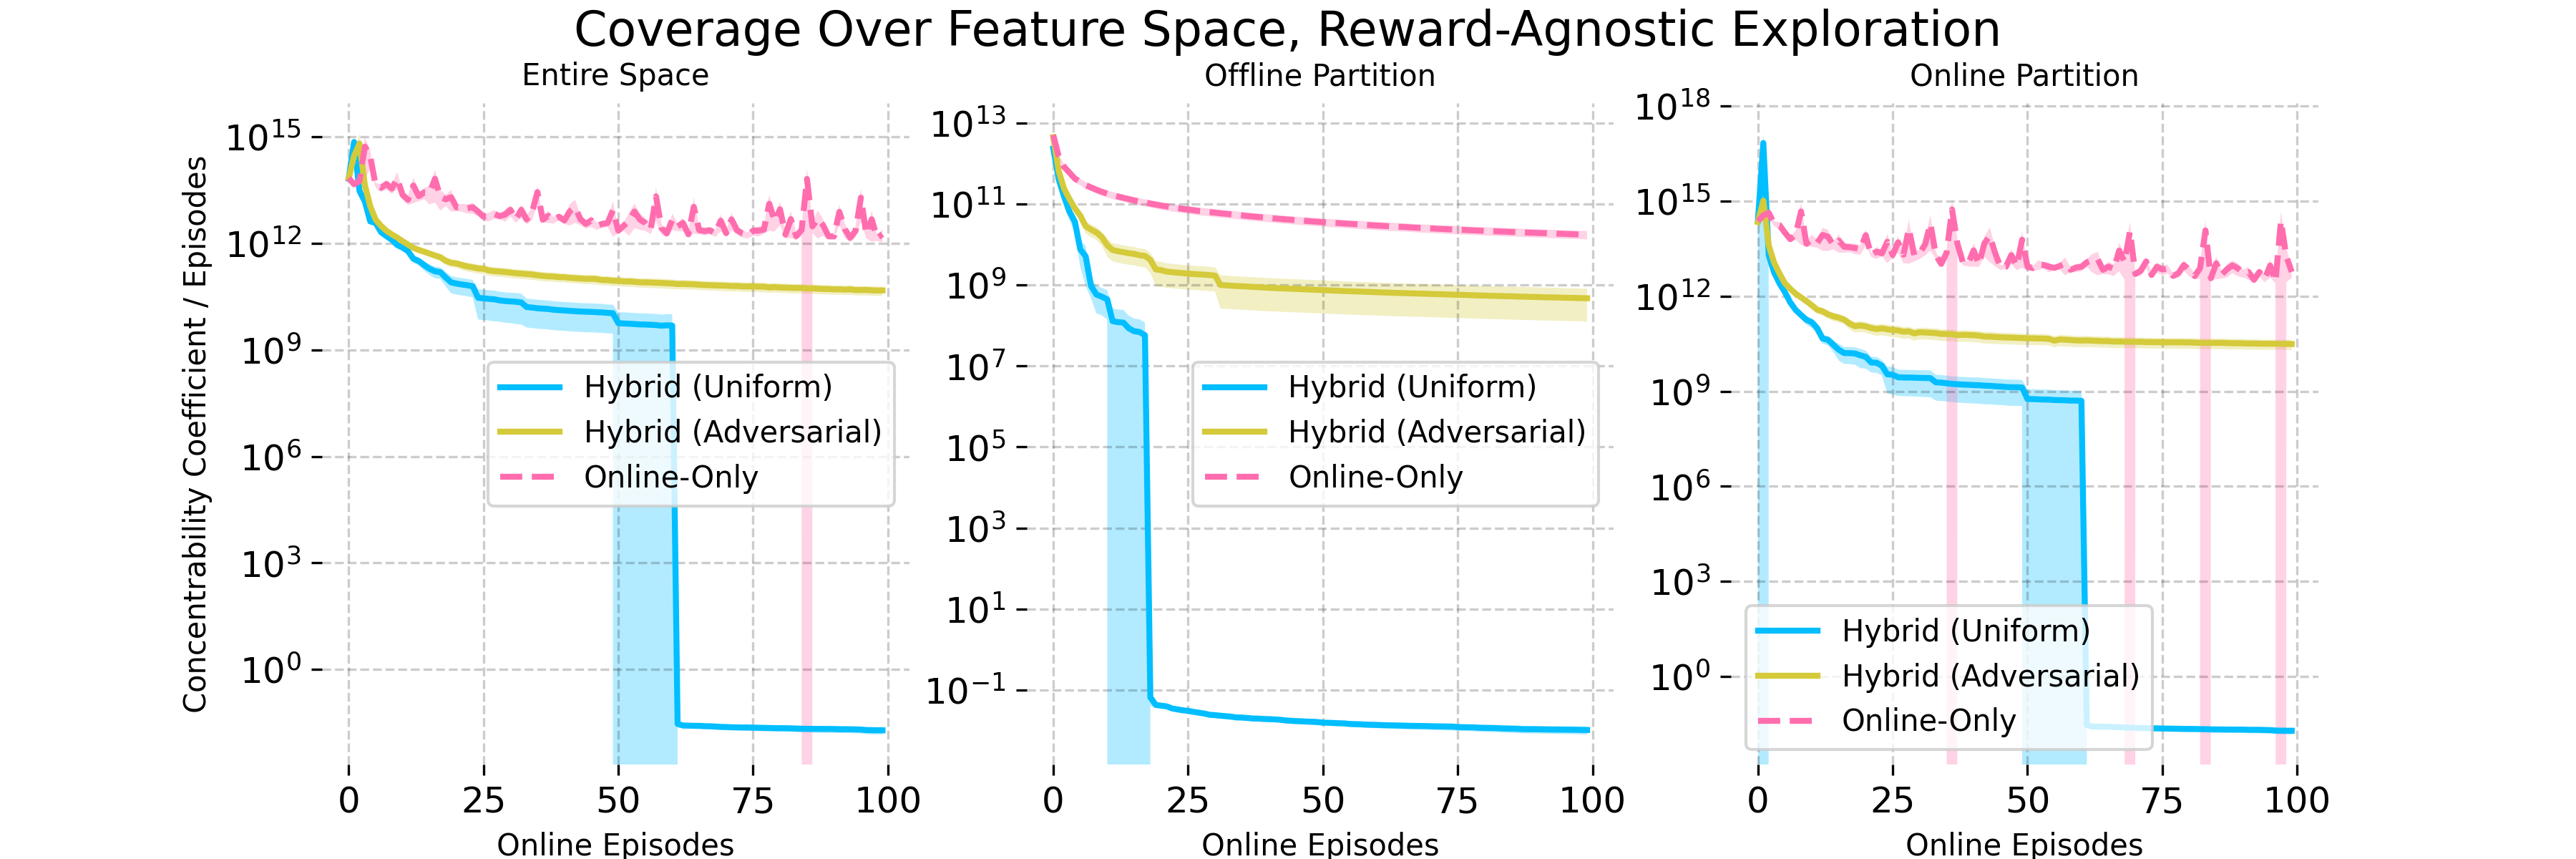
\includegraphics[width=0.95\textwidth]{figures/ch02/imgs/cov_agnostic_linear.png}
    \caption{Inverse minimum eigenvalue coverage ($1/\lambda_{\min}(\mLambda)$, $1/\lambda_{d_{\off}}(\mLambda_{\off})$, $1/\lambda_{d_{\on}}(\mLambda_{\on})$) during the reward-agnostic exploration phase of \aigen{Algorithm~\ref{alg:ch02-alg2}} initialized with 200 uniform offline trajectories, 200 adversarial offline trajectories, or no offline data (mean over 30 trials $\pm 1.96$ standard errors, where lower is better).}
    \label{fig:ch02-cov-agnostic}
\end{figure}

Figure~\ref{fig:ch02-cov-agnostic} shows the covariate coverage achieved during the exploration phase of \aigen{Algorithm~\ref{alg:ch02-alg2}} when initialized with 200 uniform-policy trajectories, 200 adversarial-policy trajectories (generated by negating the weights of a trained policy), or no offline data. Even with adversarially collected offline data, hybrid exploration achieves better conditioning across both the full space and the online subspace than purely online exploration.

\begin{figure}[htbp]
    \centering
    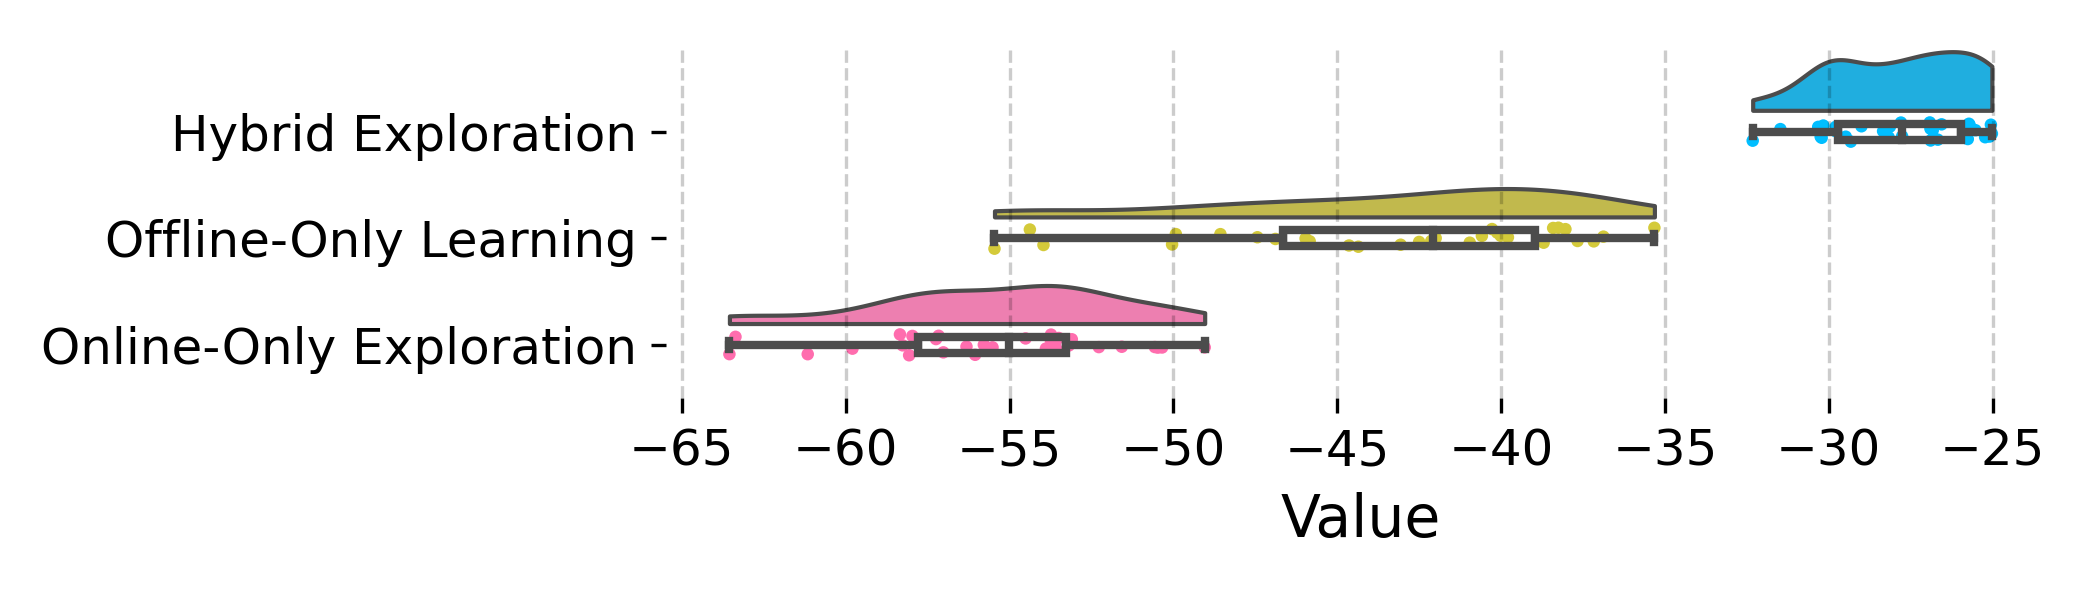
\includegraphics[width=0.52\textwidth]{figures/ch02/imgs/reward_agnostic_value.png}
    \caption{Policy value learned by pessimistic value iteration in \aigen{Algorithm~\ref{alg:ch02-alg2}} on the hybrid dataset (200 adversarial offline + 100 online trajectories) compared against 300 adversarial offline trajectories and 300 purely online reward-agnostic trajectories over 30 trials (higher is better).}
    \label{fig:ch02-reward-agnostic}
\end{figure}

Figure~\ref{fig:ch02-reward-agnostic} compares the value of the policy output by \aigen{Algorithm~\ref{alg:ch02-alg2}} using 200 adversarial offline trajectories and 100 online exploration trajectories against purely offline learning (300 adversarial trajectories) and purely online reward-agnostic exploration (300 online trajectories). The hybrid dataset yields substantially higher policy value than either pure baseline. Finally, Figure~\ref{fig:ch02-regret} compares \aigen{Algorithm~\ref{alg:ch02-alg3}} against purely online LSVI-UCB++ \citep{he2023nearly}, confirming that offline initialization yields strictly lower cumulative regret and faster reward convergence.

\begin{figure}[htbp]
    \centering
    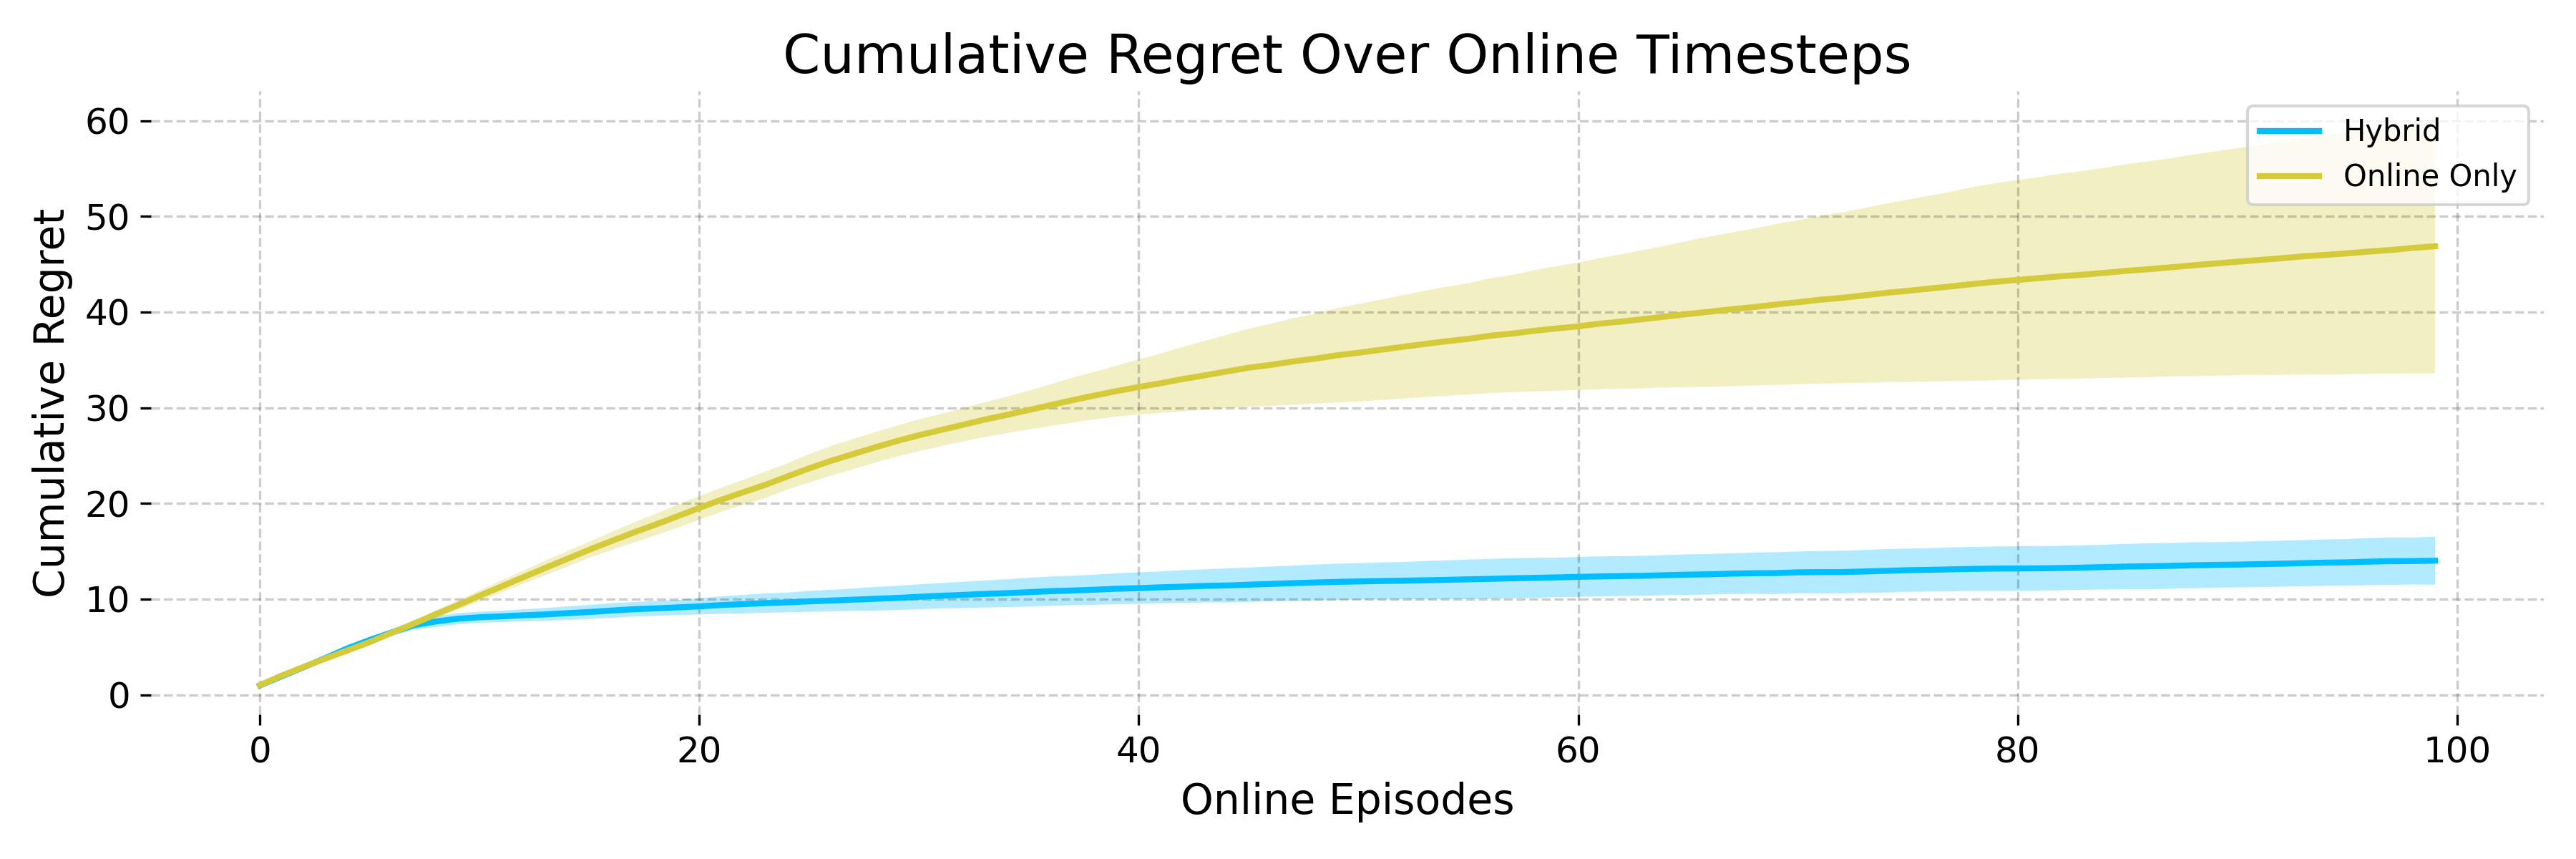
\includegraphics[width=0.78\textwidth]{figures/ch02/imgs/regret_linear.png}
    \vspace{0.1in}
    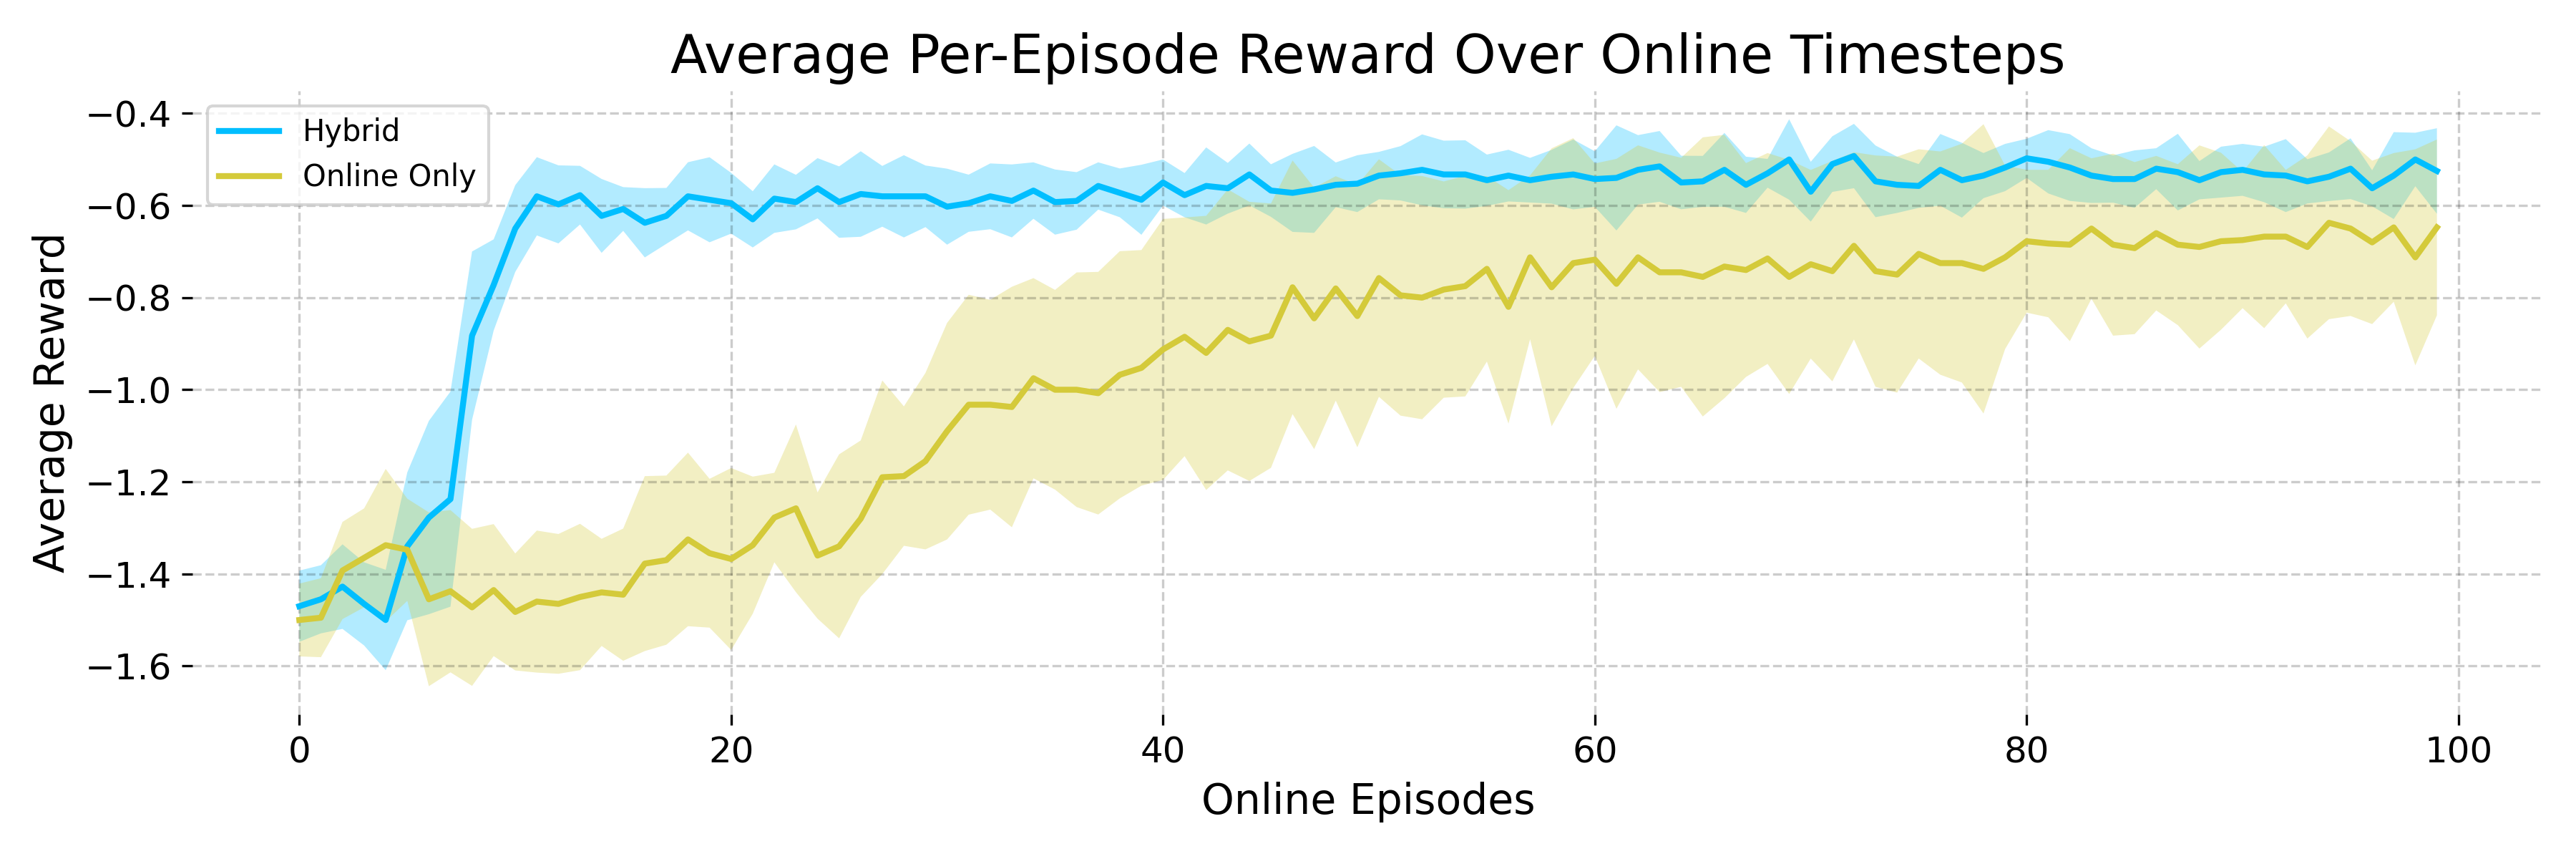
\includegraphics[width=0.78\textwidth]{figures/ch02/imgs/reward_linear.png}
    \caption{Cumulative regret (top) and per-episode reward (bottom) of \aigen{Algorithm~\ref{alg:ch02-alg3}} versus purely online LSVI-UCB++ \citep{he2023nearly} in the linear Tetris environment (mean $\pm 1$ standard deviation over 10 trials).}
    \label{fig:ch02-regret}
\end{figure}

\section{Discussion}
\label{sec:ch02-lin-discussion}

Together, Algorithms~\ref{alg:ch02-alg1}, \ref{alg:ch02-alg2}, and~\ref{alg:ch02-alg3} show that offline datasets with partial coverage can be exploited without single-policy concentrability by partitioning the state-action space into an offline-covered component $\gX_{\off}$ and an online-explored component $\gX_{\on}$. Under general function approximation, \aigen{Algorithm~\ref{alg:ch02-alg1}} achieves automatic adaptivity to the optimal partition simply by retaining the offline dataset in its experience replay buffer. In linear MDPs, Algorithms~\ref{alg:ch02-alg2} and~\ref{alg:ch02-alg3} combine this subspace decomposition with variance-weighted regression and variance truncation to achieve $H^3$ horizon dependence and $d_{\on} d$ online dimension dependence in both the online-to-offline PAC setting and the offline-to-online regret setting.

In the next chapter, we turn from learning a single decision process from partial-coverage offline data to learning shared low-dimensional representation structure across heterogeneous tasks or users in latent contextual bandits.
